% !TeX encoding = ISO-8859-1
% !TeX spellcheck = fr_FR
% !TeX root = book.tex
\documentclass[12pt, a4paper]{book}

\usepackage{graphicx}
\usepackage{geometry}
\usepackage[latin1]{inputenc}
\usepackage[T1]{fontenc}
\usepackage{xcolor}
%\usepackage[cyr]{aeguill}
\usepackage[french]{babel}
\usepackage{titlesec}
\usepackage{hyperref}


\usepackage{eso-pic}

\newcommand\BackgroundPic{%
	\put(0,0){%
		\parbox[b][\paperheight]{\paperwidth}{%
			\vfill
			\centering 
			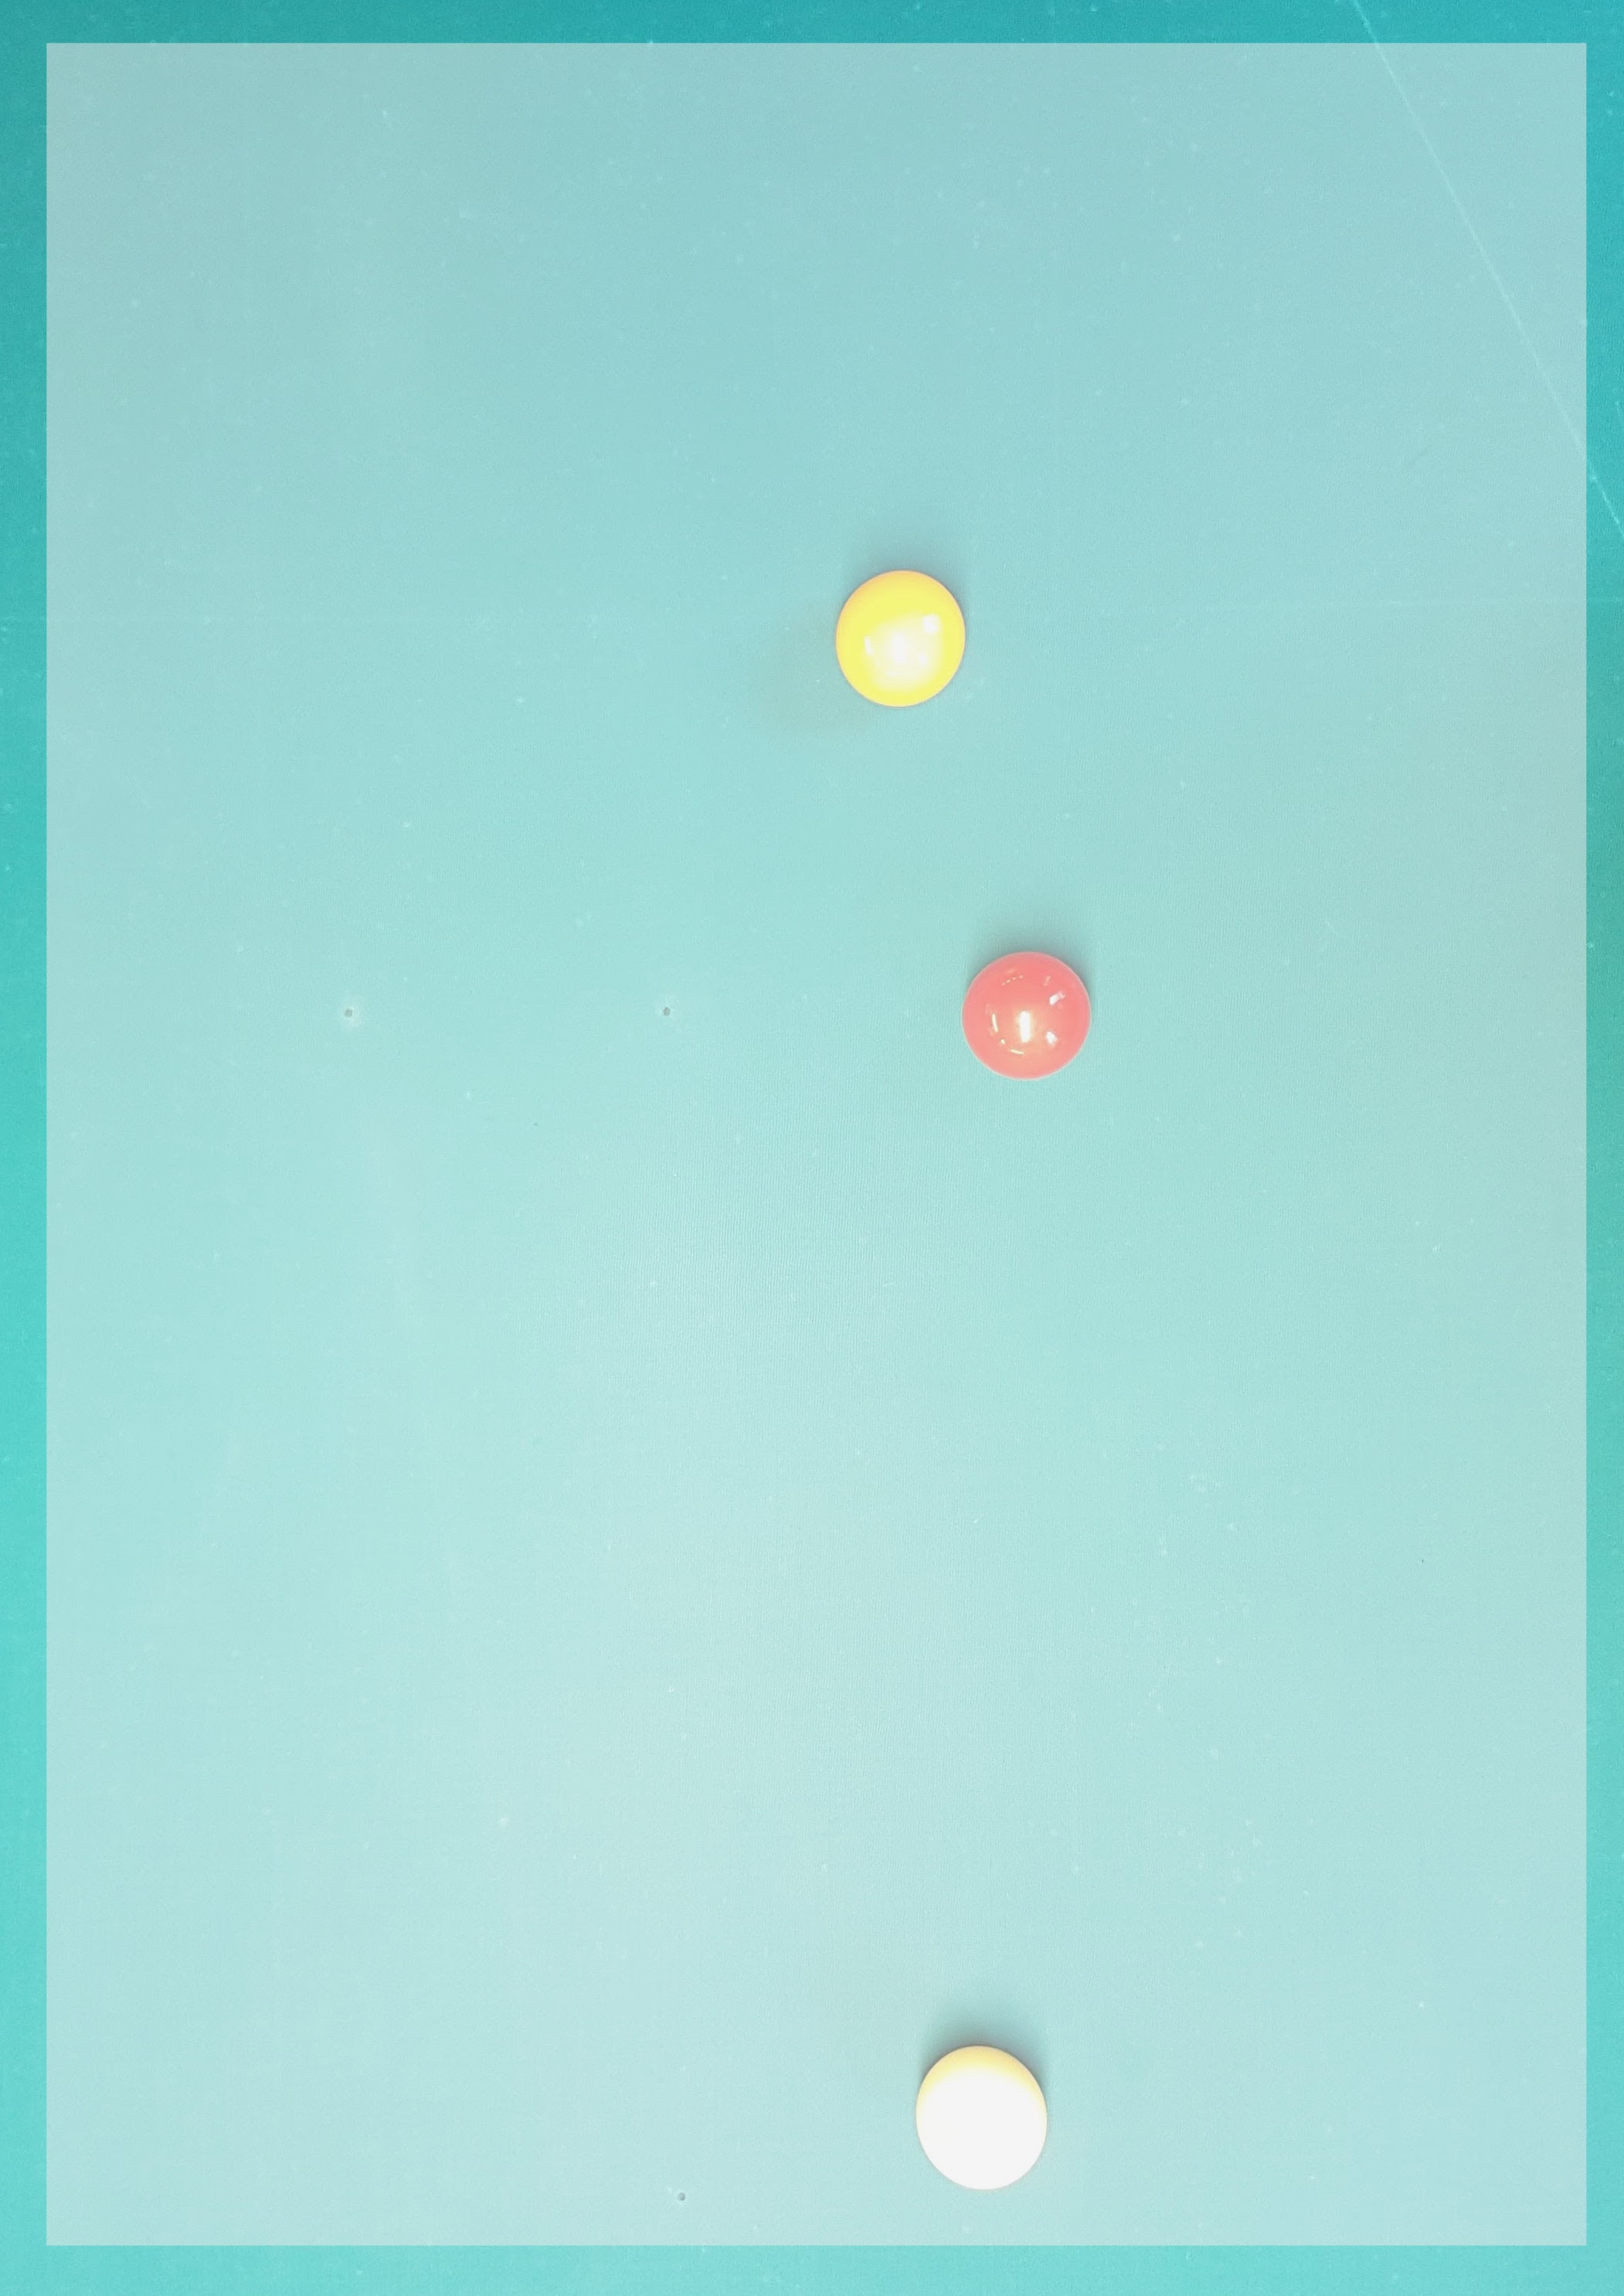
\includegraphics[width=\paperwidth,height=\paperheight,%
			keepaspectratio]{title_page_image.jpg}%
			\vfill
		}}}

%\renewcommand{\dbltopfraction}{0.9}	% fit big float above 2-col. text
%\renewcommand{\textfraction}{0.3}	% allow minimal text w. figs
%   Parameters for FLOAT pages (not text pages):
%\renewcommand{\floatpagefraction}{0.75}	% require fuller float pages
% N.B.: floatpagefraction MUST be less than topfraction !!
%\renewcommand{\dblfloatpagefraction}{0.75}	% require fuller float pages

\begin{document}
\AddToShipoutPicture*{\BackgroundPic}

\begin{titlepage}
	\thispagestyle{empty}
	\centering
	
	\textcolor{black}{\Huge{\bf Apprendre le billard au RAHB}}\\
	\Large \textbf{Andr� Gal�re}
	
	\vspace{14cm}
	
	\textcolor{black}{\Large \textit{Le Billard constitue l'Art sup�rieur de l'anticipation.	Il ne s'agit pas d'un jeu mais d'un sport artistique complet qui n�cessite une bonne condition physique,
	le raisonnement logique du joueur d'�checs et le toucher du pianiste de concert.} Albert Einstein.}
	\vfill

\end{titlepage}


\noindent Images : Pascal Allegro.\\
Edition : Bertrand Corn�lusse.\\
Avril 2023.


\tableofcontents

\chapter{Tenir sa canne}

En pr�ambule, je tiens � signaler que le cours que j'ai con�u, s'adresse aux d�butants et ne constitue qu'une m�thode. Il y en a bien d'autres. Mon but est d'aider les amateurs de billard � am�liorer leurs performances, quelles que soient la hauteur de celles-ci. Si d'aventure, quelque dou� voulait atteindre les � hautes sph�res � il conviendrait de poursuivre au-del� avec un autre cours plus sp�cialis� et un autre professeur. Ce cours devrait permettre de passer de � rien � � excellence petit format au maximum et ne permet pas de t�ter certaines disciplines comme la bande et le trois bandes. 

% !TeX encoding = ISO-8859-1
% !TeX spellcheck = fr_FR

\newpage
\section{Position du joueur}

\subsection{Les pieds} 
Les pieds doivent �tre stables, l�g�rement �cart�s de mani�re � assurer une surface au sol la plus large possible (\autoref{fig:a01-a}).
Une bonne assise permet un bon �quilibre sans d�pense d'�nergie inutile et un bon positionnement face au jeu.

\subsection{ Les jambes} 
�galement �l�ments de stabilit�, elles doivent supporter le poids du corps uniform�ment. 
Jamais, une jambe seule ne doit supporter le poids du corps, sauf s'il est impossible de poser les deux pieds au sol ! Si on doit forcer sur une jambe pour garder l'�quilibre, cela peut �tre une source d'impr�cision voire d'erreur de jugement. Les jambes doivent �tre l�g�rement fl�chies, comme si on �tait pr�t � s'asseoir sur une chaise. 
Cette position permet une orientation correcte du tronc. 
Au d�but, elle semblera un peu p�nible. 
Avec le temps, il sera possible d'am�nager des corrections de confort sans alt�rer le jugement du joueur : avancer un
pied, s'aplatir le tronc sur la canne ou raidir une jambe. \'A chacun de voir, mais retenons qu'une assise souple est toujours pr�f�rable � une assise raide.

\subsection{Le tronc} Le tronc est face � la direction choisie,
fermement stabilis�, inclin� vers l'avant. Id�alement,
le menton, le nombril et la bille 1 devraient �tre parfaitement align�s.
Seul un contorsionniste pourrait y arriver mais il faut tenter de
s'en rapprocher. Dans ses conditions id�ales, la vue du
joueur est situ�e � la verticale de cette droite (\autoref{fig:a01-b}).

\begin{figure}
	\centering
	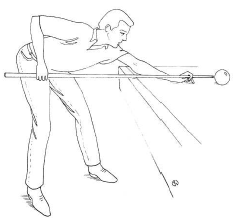
\includegraphics[width=0.7\linewidth]{A/imagesA/A01-a}
	\caption{Position du corps.}
	\label{fig:a01-a}
\end{figure}
\begin{figure}
	\centering
	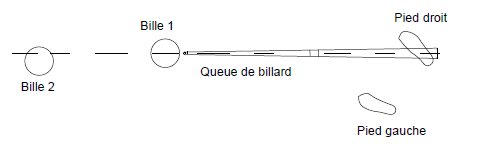
\includegraphics[width=0.7\linewidth]{A/imagesA/A01-b}
	\caption{Vue du dessus.}
	\label{fig:a01-b}
\end{figure}




% !TeX spellcheck = fr_FR
% !TeX encoding = ISO-8859-1

\newpage
\section{Position des Mains}

\subsection{La main arri�re} C'est elle qui joue ! Un gaucher a la main gauche � l'arri�re, un droitier, la main droite. Elle sert principalement � soutenir la canne, sans la presser, sans la retenir, sans la serrer. C'est cela qu'il convient d'avoir en t�te au d�but. Plus tard, nous verrons que la tenue arri�re poss�de une palette de coups et de positions. Pour l'heure, contentons-nous de bien retenir que la main arri�re soutient la canne, la fait coulisser d'avant en arri�re et d'arri�re en avant (limage), avant de porter le coup dans un mouvement r�gulier, souple, et rectiligne, bien dans le prolongement de la canne, afin d'ajuster le tir exactement, sans balancement lat�ral ni vertical. Le plus souvent possible, la canne sera mise en mouvement le plus horizontalement possible. 

\subsection{La main avant} La main avant sert � stabiliser, sans la retenir, le talon de la canne, de mani�re que celui-ci puisse coulisser sans retenue et sans jeu lat�ral. La main avant ne joue pas ! Elle ne peut pas bouger quand on porte le coup ! Elle soutient la fl�che. 

\begin{itemize}
	\item Pos�e sur le tapis, �carter bien franchement les trois doigts c�t� petit doigt, afin d'assurer une bonne assise parfaitement stable et solide (\autoref{fig:a02-3}). Le pouce sert d'appui � la canne pendant que l'index, repli� par-dessus, figure un petit pont qui va servir de serre-joint � la canne, suffisamment ferme pour emp�cher le flottement lat�ral et assez l�che pour permettre le coulissement sans retenue. De cette fa�on, on joue en position basse. Le rapprochement par arc de cercle des trois doigts de base fait passer le tir de la position basse � mi-hauteur puis � la position haute quand les doigts sont compl�tement repli�s. Pour les joueurs � � petite main �, la position haute ressemble � un poing ferm�.
	\item Pos�e sur la bande ou le bois du billard (\autoref{fig:a02-4}) : lorsque la bille � frapper est trop pr�s de la bande, emp�chant de poser la main sur le tapis, poser la canne sur le bois du billard et poser l'index et son voisin de chaque c�t� de la fl�che, doigts tendus. Serrer l�g�rement ces deux doigts de mani�re � emp�cher toute oscillation lat�rale. Dans cette position, on ne peut jouer qu'en position haute. 
\end{itemize}

\begin{figure}
	\centering
	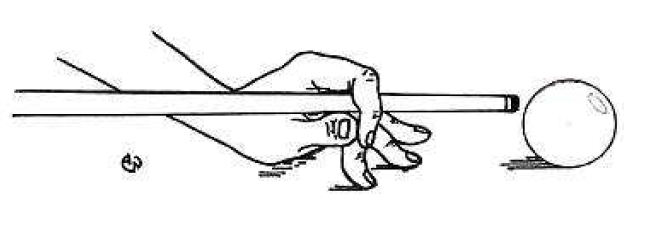
\includegraphics[width=0.48\linewidth]{A/imagesA/A02-3}
	\caption{Bille loin d'une bande.}
	\label{fig:a02-3}
\end{figure}
\begin{figure}
	\centering
	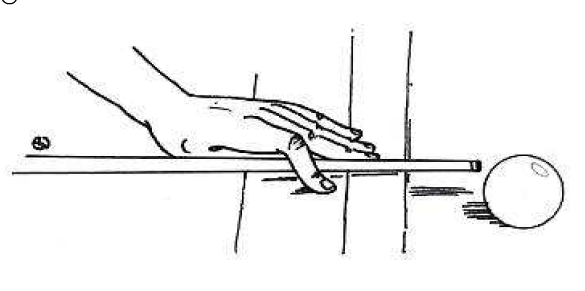
\includegraphics[width=0.48\linewidth]{A/imagesA/A02-4}
	\caption{Bille proche d'une bande.}
	\label{fig:a02-4}
\end{figure}

\noindent Remarques : 
\begin{itemize}
	\item Les deux doigts tendus sur le bois interdisent une position basse (b-2). Cependant, s'il est n�cessaire de jouer � en bas �, on devra lever le talon � l'arri�re et poser la main avant classiquement comme sur le tapis (a-1). 
	\item D'autres positions, moins fr�quentes ou plus sp�ciales, seront expliqu�es ult�rieurement. 
\end{itemize}

%TODO V�rifier 
Pour vous entrainer (\autoref{fig:a02-1}), placer les trois billes dans un coin, et frappez les de mani�re � les envoyer dans le triangle hachur� en trois bandes. La derni�re doit partir avant que la premi�re ne s'arr�te. 
\begin{figure}
	\centering
	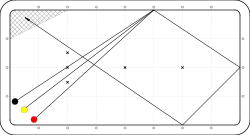
\includegraphics[width=\linewidth]{A/imagesA/A02-1}
	\caption{Envoyer les trois boules dans le coin.}
	\label{fig:a02-1}
\end{figure}

Un autre exercice (\autoref{fig:a02-2}) consiste � frapper la bille 2 pleine bille, pour que les deux billes se rencontrent apr�s le rebond de la bille 2 sur la petite bande. Cela permet d'apprendre � frapper bien droit.
\begin{figure}
	\centering
	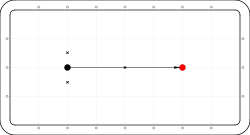
\includegraphics[width=\linewidth]{A/imagesA/A02-2}
	\caption{Frapper droit.}
	\label{fig:a02-2}
\end{figure}


% !TeX spellcheck = fr_FR
% !TeX encoding = ISO-8859-1

\newpage
\section{L'effet : position de la canne}

La canne est compos�e principalement d'un talon, d'une fl�che, d'une v�role et d'un proc�d�. Nous jouons en projetant le proc�d� (le cuir) sur la bille. La 1 est la bille avec laquelle nous jouons, la 2, celle qui sera percut�e la premi�re par la 1 et enfin la 3, la derni�re touch�e par la 1. Le jeu consiste, en � libre �, � frapper la 1 avec le cuir de notre fl�che de mani�re qu'elle aille percuter les deux autres billes. 

Chaque � coup � r�ussi est compt� un point par l'arbitre et permet de continuer le jeu tant qu'on r�ussit, pouvant ainsi � marquer � plusieurs points avant de passer la main. Si on rate au premier essai, l'arbitre compte z�ro et on doit passer la main � l'adversaire directement. Une partie se joue en un certain nombre de points � r�aliser allant de la huiti�me cat�gorie (30 points) � l'excellence (300 points). 

De mani�re � ex�cuter une carambole correspondant � une vision directe, il est important pour la majorit� des points que la canne soit tenue le plus pr�s possible de l'horizontale. Avant tout : limer. La pr�cision est essentielle. Pour cela, il conviendra de rep�rer sur la bille, des endroits bien d�termin�s qui, avec un coup toujours le m�me, donnera un r�sultat, toujours le m�me (\autoref{fig:a03-1}). 
Si on partage la 1 par deux axes, l'un vertical et l'autre, horizontal, on partage le cercle visible de la bille en 4 zones ou secteurs. Nous d�gageons ainsi, 9 prises de billes pr�cises � savoir : 

% TODO v�rifier figure d'Andr�.
\begin{itemize}
	\item Au croisement des deux axes pr�cit�s ou centre bille ou au milieu de la distance entre le centre et le haut ou au milieu de la distance entre le centre et le bas, soit sur l'axe vertical : on joue sans effet (la bille ne tourne pas sur elle-m�me pendant sa translation). 
	\item Jouant au centre de la zone 1, on imprime un effet � gauche faible. Pendant sa translation, la bille tourne sur elle-m�me faiblement dans le sens des aiguilles d'une montre. 
	\item Le coup port� au milieu entre le centre et l'extr�mit� gauche (ou au milieu entre le centre et l'extr�mit� droite, donc sur l'axe horizontal, imprimera un effet important. 
	\item 	Enfin, au milieu du secteur 3, l'effet port� sera tr�s important. 
	\item 	Les zones 2 et 4 sont �quivalentes aux zones 1 et 3, l'effet est port� � droite. 
\end{itemize}
\begin{figure}
	\centering
	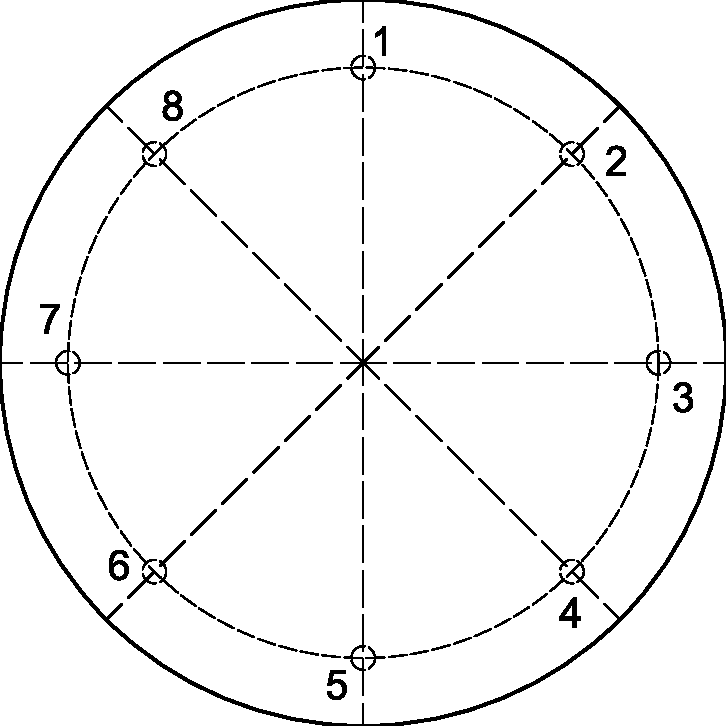
\includegraphics[width=0.4\linewidth]{A/imagesA/A03-1.pdf}
	\caption{Les positions de frappe sur une bille.}
	\label{fig:a03-1}
\end{figure}

\begin{figure}
	\centering
	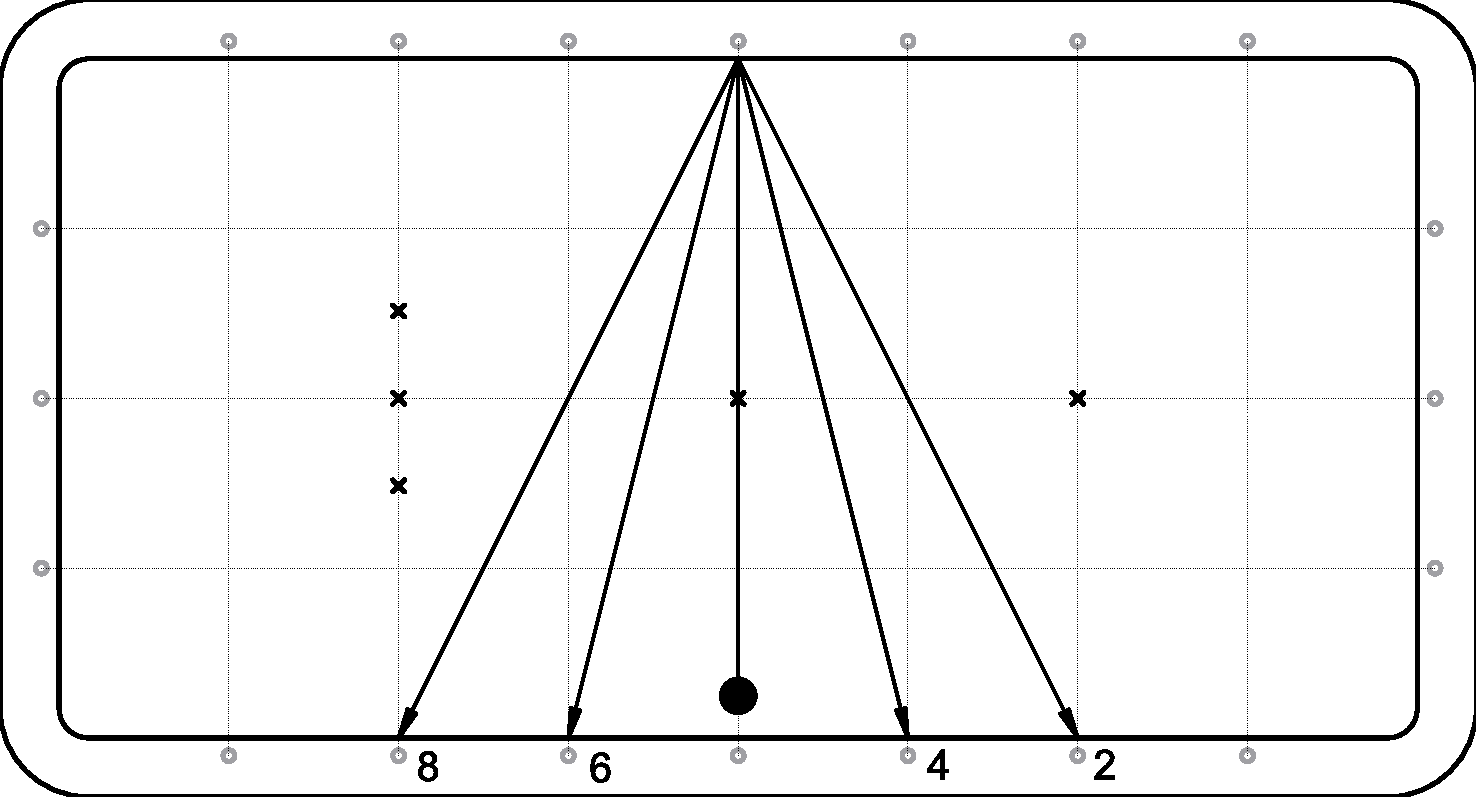
\includegraphics[width=0.95\linewidth]{A/imagesA/A03-2.pdf}
	\caption{Exercice sur l'effet � gauche et � droite. Essayez de doser l'effet lat�ral en partant du centre du billard et en suivant la perpendiculaire � la grande bande afin d'atteindre les points 2, 4, 6 et 8.}
	\label{fig:a03-2}
\end{figure}
\noindent Essayez l'exercice de la \autoref{fig:a03-2}.
\begin{itemize}
\item L'effet produit son << effet >> seulement (ou � peu pr�s) lorsqu'il rencontre un obstacle, par ex.la bande. 
\item On appellera � bon effet �, celui qui a tendance � prolonger le mouvement de la bille o�, apr�s contact, la bille se rapproche de la bande.
\item On appellera � effet contraire �, celui qui a tendance � contrecarrer le mouvement de la bille, o�, apr�s contact, la bille se rapproche de la perpendiculaire � la bande. 
\item Cette d�signation de bon effet ou effet contraire est pure convention pour cet expos�.  D'autres d�signent les choses autrement : question de convention afin de se comprendre par la suite. 
\end{itemize}
\clearpage


% !TeX spellcheck = fr_FR
% !TeX encoding = ISO-8859-1

\section{L'effet}

Le � bon effet � prolonge le mouvement de la bille, l' � effet contraire
� ralentit le mouvement de la bille, voir \autoref{fig:a04-1}. L'effet ne produit son effet qu'en rencontrant un obstacle.
Les changements de direction dus � l'effet seront d'autant plus
importants qu'on jouera bas de bille.

Fig l : L'effet est contraire sur la bille 2 et bon sur la bande : la
1 aura tendance � s'�tendre le long de la bande donc � s'�carter de la
perpendiculaire au point d'impact sur la bande, ou, si l'on pr�f�re :
l'angle de r�flexion sera plus grand que l'angle d'incidence.

Fig 3: L'effet est bon sur la bille 2 et contraire sur la bande. La 1 aura tendance � retenir son mouvement donc � se rapprocher de la
perpendiculaire � la bande au point d'impact : l'angle r�fl�chi sera
plus petit que l'angle d'incidence.

Fig 2 : Cette figure montre le ph�nom�ne d'engrenage de l'effet. Tout se passe comme si les billes �taient des roues dent�es. Quand la 1
rencontre la deux, elle lui donne une partie de son �nergie sous forme
de rotation dont le sens sera inverse � celui d'origine ... comme avec
les engrenages. 
\begin{itemize}
\item Ainsi, si nous imprimons � la 1 une rotation gauche, au moment de l'impact avec
la 2, elle imprimera � celle-ci une rotation droite. L'effet de la 2
sera plus faible que celui d'origine mais pas du tout inexistant. On
constatera le ph�nom�ne de deux fa�ons : la 2 est l�g�rement d�vi�e dans
le sens de l'effet de la 1 et au toucher de la premi�re bande, elle aura
une d�viation correspondant � l'effet inverse de la 1.
\item C'est en � soutenant � bien son � coup � qu'on imprimera une
part plus importante d'effet � la 2. Ce ph�nom�ne d'engrenage est
capital pour rappeler des positions qui sans cela, seraient perdues. La
bonne compr�hension de ce ph�nom�ne facilitera grandement l'�tude du jeu
de rappel.
\end{itemize}

\begin{figure}[htb]
	\centering
	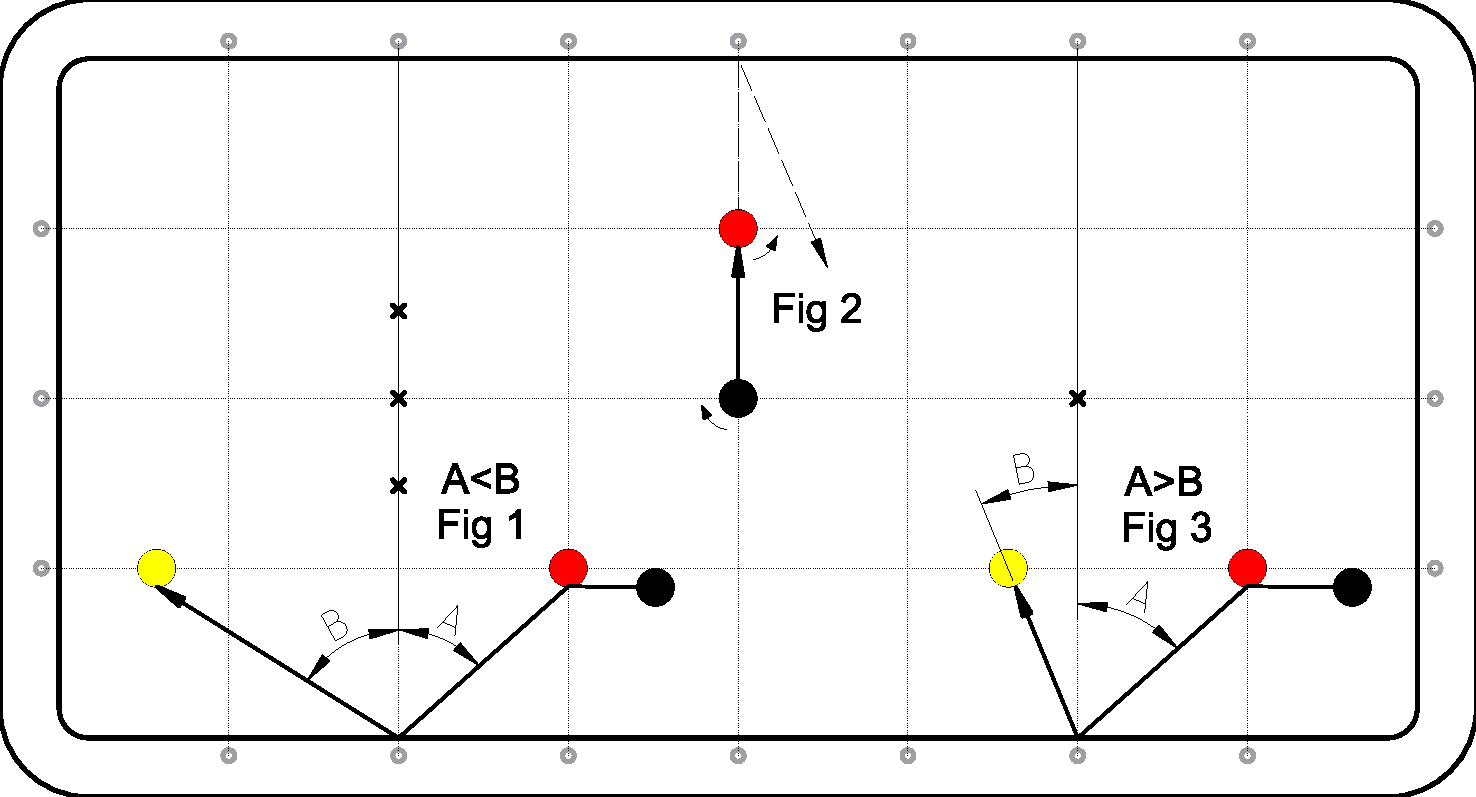
\includegraphics[width=\linewidth]{A/imagesA/A04-1.pdf}
	\caption{Effet contraire, engrenage et bon effet.}
	\label{fig:a04-1}
\end{figure}

\clearpage
% !TeX spellcheck = fr_FR
% !TeX encoding = ISO-8859-1

\section{Le coul�}

Le coul� (\autoref{fig:a05-1}) est un des points de base du billard. Il permet de r�aliser des caramboles dites <<non naturelles>>.

La bille 2 est plac�e de telle sorte que la finesse est impossible ou
tr�s difficile. D'abord examinez si le coul� est possible. Celui-ci
consiste � faire prolonger le mouvement de la 1 vers l'avant apr�s avoir
heurt� la 2, parfois presque la m�me direction comme si la 1 voulait
suivre la 2. Mais pour que le point soit possible, la direction 1-2 ne
peut pas � couper � l'image de la 3, sinon apr�s le coup, la 2 risque de
toucher la 3 et l'�carter emp�chant ainsi la 1 de r�aliser le point.
Pour v�rifier cela : tracez une ligne imaginaire tangente aux billes 1
et 2, c�t� de la 3 et si cette ligne ne rencontre pas la 3, le point est
possible.

Le coul� � normal � se joue presque plein sur la 2, coup prolong�, haut
de bille, coup accompagnant la 1 dans son mouvement. Le d�calage de la
prise de la 1 se situe du c�t� de la 3. La masse non prise de la 2,
correspond � la touche qu'on aurait d� n�gocier si on avait tent� la
finesse. Autrement dit, il faut prendre � toute � la 2 moins ce qu'on
aurait pris en finesse. Une l�g�re d�portation sera donc appliqu�e du
c�t� de la 3. Lorsque la prise de la deux est particuli�rement proche de
la bille pleine, on parlera d'une nuance droite pour une d�portation
vers la droite et d'une nuance gauche pour une d�portation vers la
gauche.

Le coup � normal � se porte sur l'axe vertical, donc sans effet.
Beaucoup de joueurs croient faciliter le coul� en appliquant un effet
inverse � la d�portation. Cela est pure l�gende. L'effet impliqu� jouera
dans le cas o� nous coulons vers la bande ou bien imprimera un effet
inverse � la 2. L'effet n'influence pas le mouvement de la 1 ... ou si
peu.... Il rassure, c'est tout. En fait, l'effet inverse rapproche la 2
du champ de la 3, l'effet du bon c�t� l'�carte.

Nous allons nous servir de cette qualit�. Si la tangente cit�e plus haut
� mord � un peu la 3, sans exag�ration, il sera encore possible de
r�aliser le coul�. On appliquera un effet du c�t� de la d�portation et
la 2 s'�cartera du chemin de la 3 (� essayer).

Si la tangente passe trop pr�s du centre, la d�viation de la 2 ne sera
jamais suffisante pour �viter le choc avec la 3. Il conviendra d�s lors
de choisir une autre solution.
\begin{figure}[htb]
	\centering
	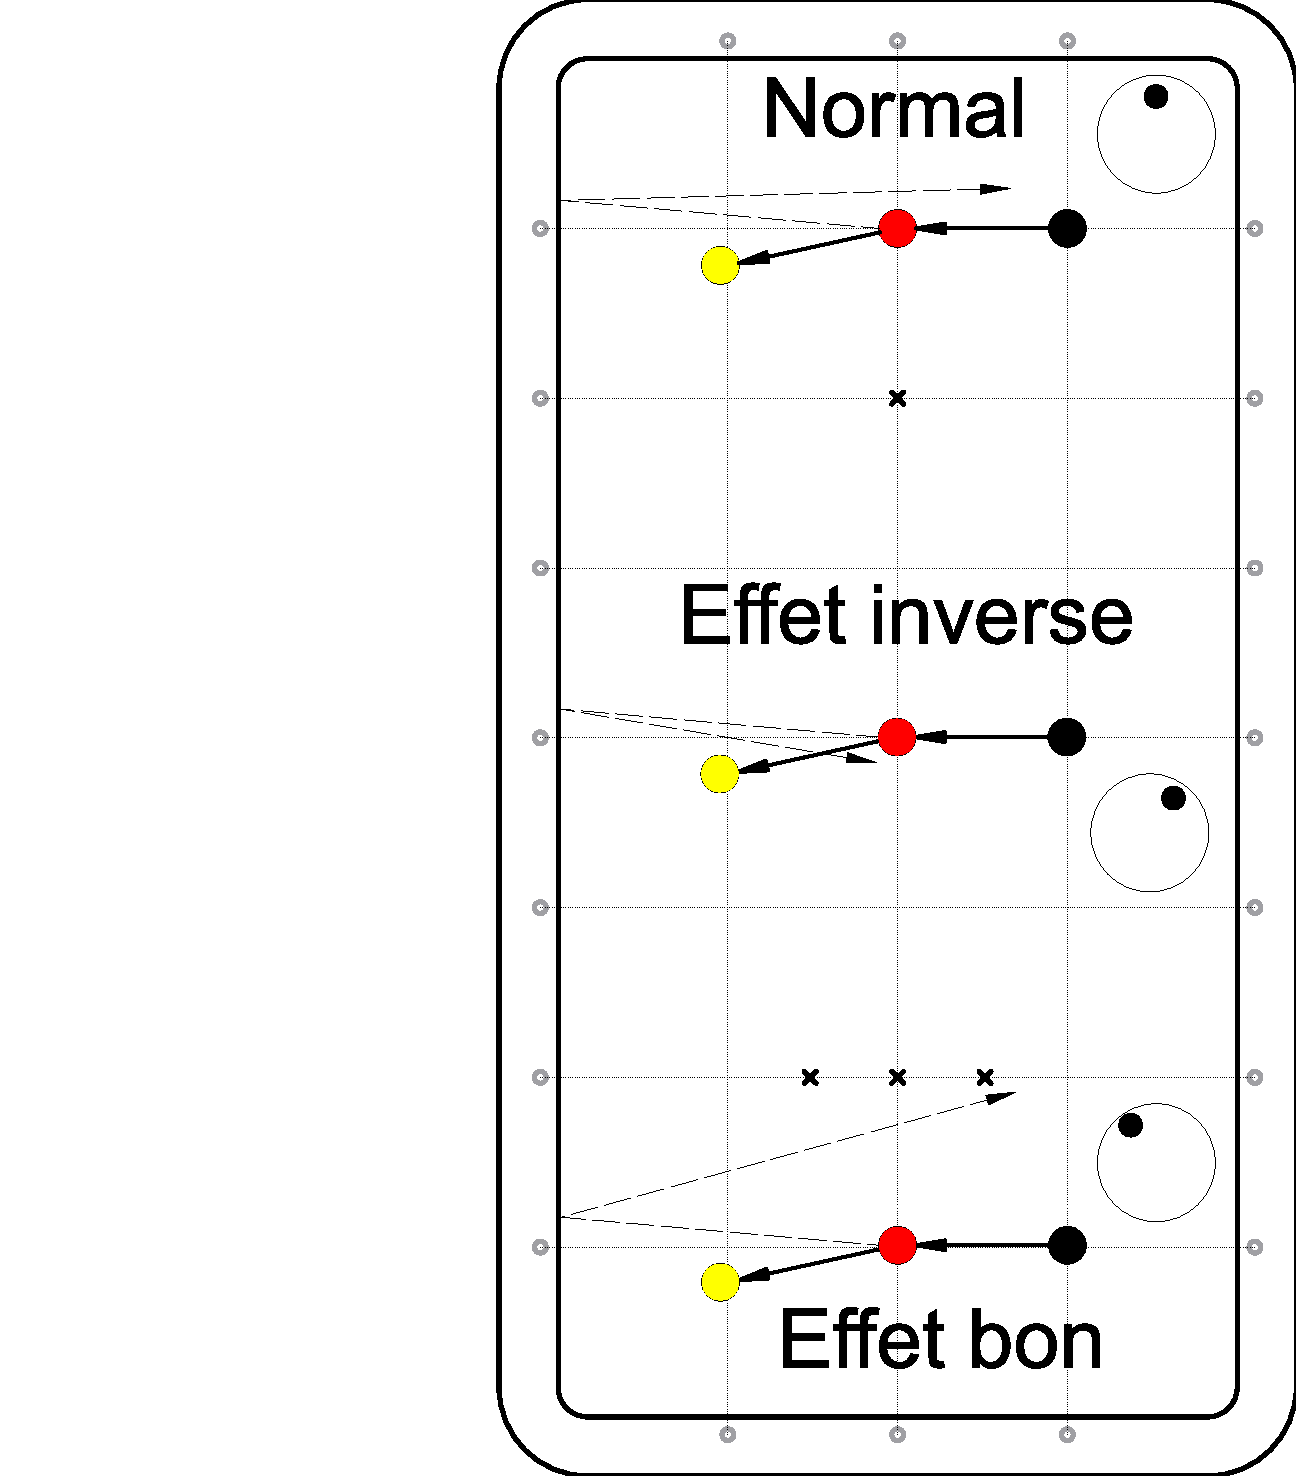
\includegraphics[width=0.85\linewidth]{A/imagesA/A05-1.pdf}
	\caption{Le coul�.}
	\label{fig:a05-1}
\end{figure}
\clearpage

% !TeX spellcheck = fr_FR
% !TeX encoding = ISO-8859-1

\section{Le r�tro}

Le r�tro est aussi un point de base au billard. Sa r�alisation est
facile pour un joueur aguerri mais ardu pour un d�butant. Il faudra
s'acharner jusqu'� ce que la � m�canique � devienne une <<�vidence>>.

Le r�tro est le contraire du coul�. La bille 1 revient sur ses pas en
direction de la 3, apr�s avoir touch� la 2. Il se joue bille basse, coup
allong� et m�me accompagnant, l�che et sans forcer. La main avant est
ferme et laisse une fl�che courte pour les petits d�placements et une
fl�che longue pour les longs. La main arri�re ne serre pas le talon et
se place le plus loin possible pour les longs d�placements et se
rapproche de l'�quilibre de la canne pour les petits points. La grosseur
de bille est la m�me que pour le coul� mais on y voit bien plus mal. Son
estimation ne sera pas chose ais�e aussi, nous allons utiliser un truc.

Consid�rons la fig 2 et voyez l'angle form� par les billes 1, 2 et 3,
sommet en 2... Tra�ons la bissectrice de cet angle qui coupe la surface
de la 2 au point I. Il suffit (hum...) de jouer sur ce point I et le
tour est jou�. Facile � dire car le point I est le point de touche et
pas celui de la vis�e mais rien n'est perdu car les billes sont des
miroirs sph�riques donc si nous nous positionnons pour jouer un r�tro,
nous allons voir dans la 2 l'image de la 3 ... et en visant cette image,
nous allons toucher au point I recherch�.

Merveille de la g�om�trie sph�rique !

Nous n'avons donc plus besoin de nous torturer pour mesurer la grosseur
de bille ... si la 2 est la rouge. Nous voyons bien l'image et m�me si
la 3 est �loign�e, son image est encore un petit point qu'on peut
apercevoir. Malheureusement, si la 2 est la blanche, nous ne voyons plus
l'image de la 3. Il conviendra de s'entra�ner ferme pour se � mettre
dans l'�il � cette fameuse grosseur de bille. Tout ceci est un truc et
n'est valable seulement que si on ne fait pratiquement intervenir que
les masses des billes c�d : bille basse, sans effet, p�n�tration moyenne
; force moyenne et main arri�re en position moyenne.

Attention ! la position et la tenue de la canne par la main arri�re sont
capitales. Afin d'assurer un bon retour de la 1, la main arri�re ne doit
que soutenir la canne, sans la presser. Pour ce coup, � la limite, on
pourrait se passer de cette main, elle est presque inutile. Il ne s'agit
pas d'une contradiction : la main arri�re est indispensable mais elle
doit se faire l�g�re.... presque gracieuse...

Remarque : Il y d'autres trucs mais c'est celui-ci que je pr�f�re... Il
a l'avantage, je crois, de forcer le joueur � toujours produire le m�me
coup ce qui, plus tard, lui permettra de bien le dominer, donc de le
varier et de lui permettre de dominer le mouvement de la 2 autant que
celui de la 1, donc de � construire � son jeu.

\begin{figure}[htb]
	\centering
	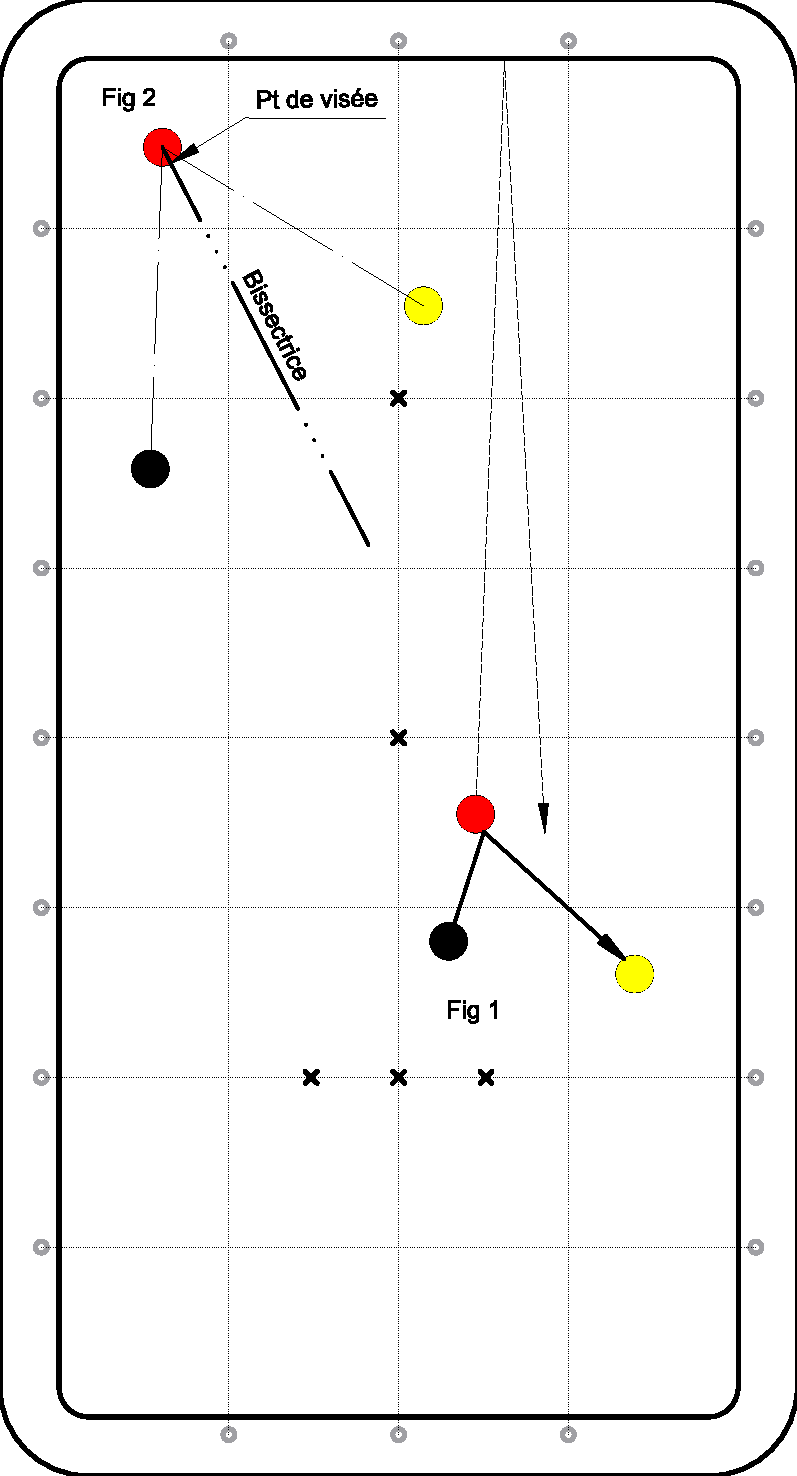
\includegraphics[width=0.85\linewidth]{A/imagesA/A06-1.pdf}
	\caption{Le r�tro}
	\label{fig:a06-1}
\end{figure}
\clearpage

%% !TeX spellcheck = fr_FR
% !TeX encoding = ISO-8859-1

\section{Le 45�}

Ce point est particuli�rement important dans la mesure o� il constitue
une r�f�rence pour beaucoup de figures. Une fois acquis, il ne peut plus
�tre rat� (!). Il est facile. En cas d'�chec, notre ?il ou notre
position est responsable, voire notre distraction...

Il suffit de jouer en demi-bille la 2 du c�t� de la 3. � Prendre � une
demi-bille, c'est pousser la 1 en direction de la 2 de mani�re que, dans
son mouvement, la moiti� de la masse de la 1 co�ncide avec la moiti�
oppos�e de la masse de la 2... Pour une vis�e pr�cise, la 1 est prise au
centre bille, avec comme point de vis�e, la tangente � la 2. Il suffit
pour cela, une fois bien positionn�, de placer dans � sa vis�e �, le
bord de la 2 au milieu de l'image de la mouche de la fl�che.

Apr�s l'impact, la 1 ferait un angle de 45� si nous �tions dans un
espace � trois dimensions et sans frottement et si les billes 1 et 2
�taient en mouvement libre l'une vers l'autre et � vitesse �gale. Mais
comme nous sommes avec des volumes glissant sur un plan et qu'en plus le
mobile percuteur est en mouvement quand il s'�crase sur sa cible fixe et
... qui va se d�rober, l'angle est un peu inf�rieur, jusqu'� 40� si la
canne est tenue haute comme pour couler et jusqu'� 50� si la canne est
soutenue l�g�rement basse.

Retenons qu'une demi-bille a pour r�sultat un angle de 45�. Il y a une
erreur mais petite. En plus avec l'habitude, la merveilleuse m�canique
humaine va ajuster sans peine, ces petites diff�rences.

\begin{figure}[htb]
	\centering
	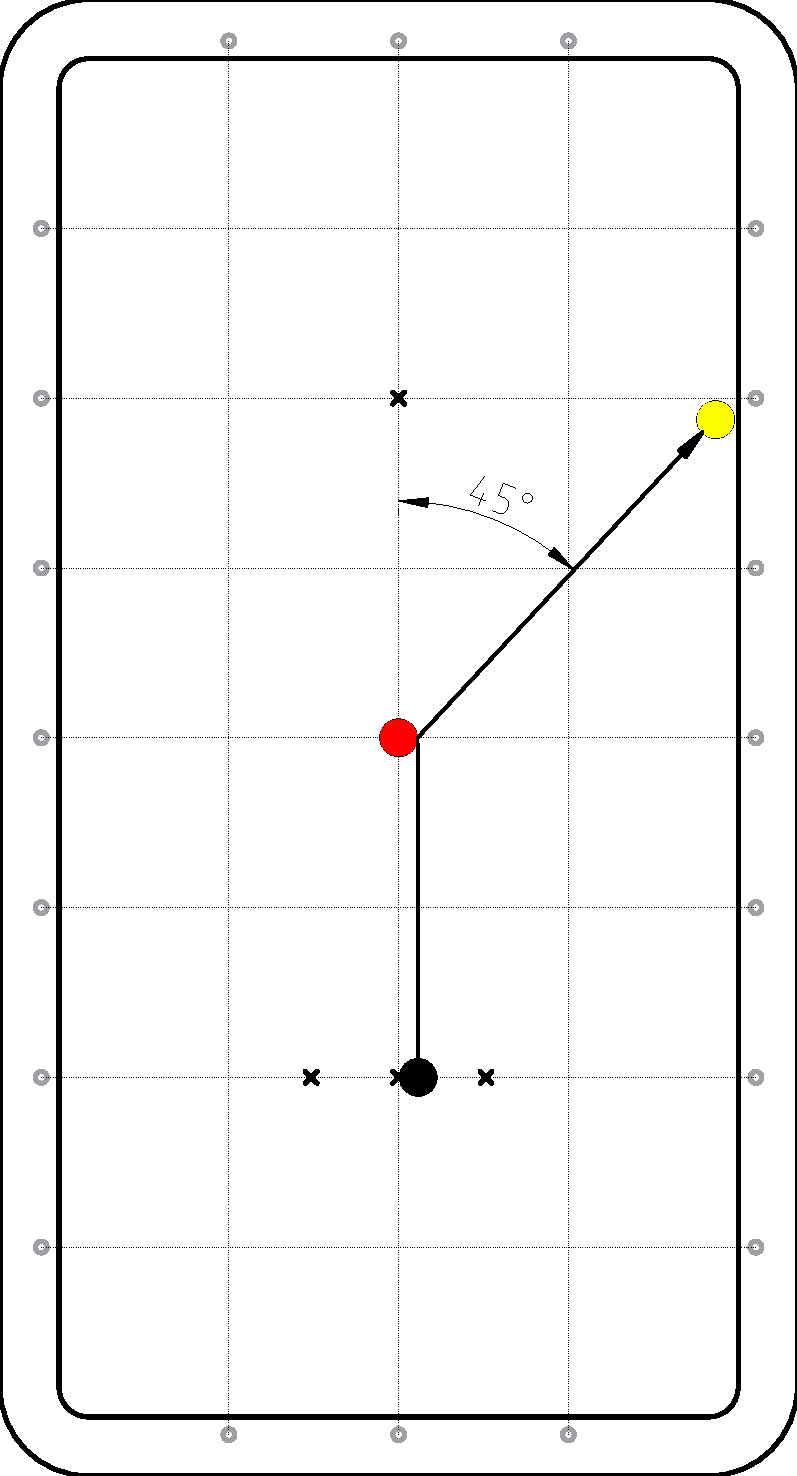
\includegraphics[width=0.85\linewidth]{A/imagesA/A07-1.pdf}
	\caption{Le 45�}
	\label{fig:a07-1}
\end{figure}
\clearpage

%% !TeX spellcheck = fr_FR
% !TeX encoding = ISO-8859-1

\section{Le 90�}

Le 90� ou angle droit constitue un pas important � franchir pour le
d�butant. Bien travaill�, ce point devient facile, croit-on... M�fiance,
il est plein de nuance. Les � sp�cialistes � diront qu'on peut r�aliser
un angle droit aussi bien bon effet que contraire, qu'une prise de bille
pleine ou fine, voire superfine. Nous nous bornerons ici, � une m�thode,
laissant pour le futur, les particularit�s et les coups d'�clat...

Nous choisirons de jouer le 90� par 3/4 bille, fl�che basse, au milieu
du secteur inf�rieur c�t� bille 3 ou bien milieu du demi-axe inf�rieur.
Nous essayerons le milieu de secteur, l'exp�rience r�v�lant que le
joueur se rassure et est plus pr�cis avec cette m�thode. Le coup est
moyennement allong� et souple. C'est un proche parent du r�tro.
Attention ! Il est faux de croire que l'effet aide � la r�alisation.
Contrairement � certaines id�es re�ues, l'effet rassure et vaut
�ventuellement pour la � rentr�e � de la 2, c�d pour remettre la 2 dans
une position rapproch�e.

Nous nous entra�nerons de cette mani�re. La description pr�c�dente est
cependant une position moyenne. Les limites de la prise de la 2 sont
�tendues. Si on prend seulement un peu plus qu'une demi-bille, le coup
sera souple et allong� et un peu plus bas comme un v�ritable r�tro. Si
on prend un peu plus que 3/4, on jouera un peu plus haut sur l'axe
central tout en restant sous le centre ou bien on se rapprochera du
centre si on avait choisi le secteur. Si on prend la 2 pleine, avec
seulement une nuance du c�t� o� on veut d�porter, le coup sera un peu
plus rude, plus court et la fl�che se rapprochera du centre bille.

Remarques :

\begin{itemize}
	\item
	Le conseil est de d'abord essayer la m�thode du � secteur �, apr�s il
	sera encore temps de tenter des choses plus difficiles.
	\item
	Plus la bille 2 sera prise grosse, plus le mouvement de la 1 sera
	ralenti et celui de la 2, acc�l�r�. Plus la bille 2 sera prise fine,
	plus le mouvement de la 1 sera rapide et celui de la 2, ralenti.
	\item
	Le � transfert � d'�nergie entre les billes 1 et 2 est proportionnel
	aux masses en contact dans le couloir de percussion et � la hauteur de
	la prise de la 1.
	\item
	C'est en dosant ces diff�rents �l�ments qu'on se m�nage des positions
	favorables ou non. N'oublions pas que l'effet sert (presque) seulement
	� diriger la 2 !
\end{itemize}

\begin{figure}[htb]
	\centering
	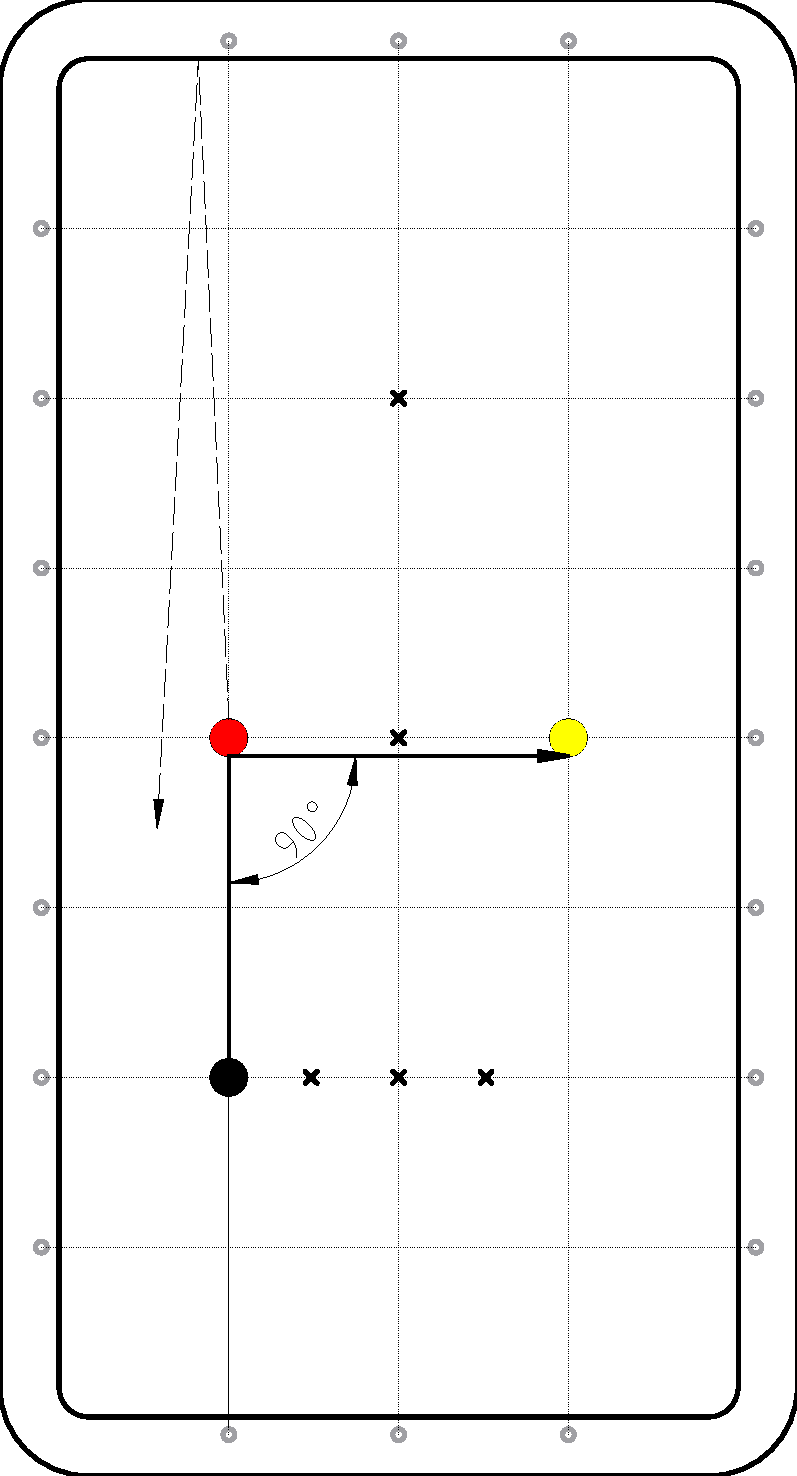
\includegraphics[width=0.85\linewidth]{A/imagesA/A08-1.pdf}
	\caption{Le 90�}
	\label{fig:a08-1}
\end{figure}
\clearpage

%% !TeX spellcheck = fr_FR
% !TeX encoding = ISO-8859-1

\section{Bosse sur la bille colleuse}


Quoique ce point n'est g�n�ralement tent� que quand le 1bande est
difficile ou impossible, il constitue maintenant un bon exercice de
ma�trise qui nous servira et nous suivra m�me jusqu'en cinqui�me ann�e
o� il va contribuer � l'apprentissage du point dit � � l'Am�ricaine
\textgreater{}\textgreater{} car il donne le pouvoir de bien contr�ler
la 2 le long d'une bande.

La 2 collant la bande fait corps avec elle. Elle va nous servir de
rebond pour la 1. Comme la 1 rencontre une forme circulaire au point
d'impact (de m�me mesure qu'elle), l'angle de r�flexion sera le double
de l'angle d'incidence. Pour �valuer la grosseur de bille � � prendre �,
on peut appliquer la r�gle du r�tro (image de la 3 dans la rouge). On
peut aussi calculer cette prise en L 3 imaginant une petite construction
: Tracer mentalement une droite reliant les billes 1 et 2. Tracer une
perpendiculaire � cette droite passant par le centre de la 2. Consid�rer
la bille 3', image sym�trique de la 3 par rapport � la perpendiculaire
cit�e. Ne regardons plus maintenant la 3 mais la 1, la 2 et la 3'... Il
ne reste plus qu'� appliquer un simple coul�. Cette technique semble
tr�s compliqu�e sur le papier mais l'est beaucoup moins sur le tapis...
Elle donne cependant une l�g�re erreur mais insuffisante pour rater le
point tant que l'angle de r�flexion n'exc�de pas 45�.

Attention : jouer sans effet ! (fig. 1) Pr�caution : malgr� l'attention
qu'on y apporte, la 2 colle rarement la bande. Le moindre espace modifie
la donne. Il sera prudent d'appliquer une nuance plus pleine ou bien un
petit effet contraire. � essayer sur place !

Si on applique un effet quelconque, la trajectoire de la 1 peut s'en
trouver tr�s chang�e.

\begin{itemize}
	\item
	Effet � gauche : prendre la 2 un peu plus fine : celle-ci � avance �
	vers le jeu.
	\item
	Effet � droite : prendre la 2 un peu plus grosse : celle-ci se d�colle
	sans avancer.
	\item
	Prise de bille haute : la 2 reste � �cras�e � (coll�e) sur la bande.
	Le mouvement de la 1 est ralenti.
	\item
	Prise de bille basse : la 2 se d�colle. Le retour de la 1 est rapide.
	\item
	Figure 2 : c'est un angle droit. Appliquons un angle de 45�, celui de
	retour sera de 90�. A cause de � l'�crasement de la 2 sur sa bande, la
	pratique montrera qu'une prise un peu plus grosse que la demi-bille
	assure mieux...
	\item
	Dernier cas : si la 2 ne colle pas la bande : Ne visez plus l'image de
	la 3 dans la rouge mais bien un point plus proche du centre de la 2.
	Ce point devrait �tre calcul� en partant de ladite image et en entre
	la distance de la 2 � sa bande proche. Attention, si cette distance
	porte le point de vis�e au-del� du centre, le point-bosse n'est plus
	possible. Il faut choisir une autre solution.
\end{itemize}

\begin{figure}[htb]
	\centering
	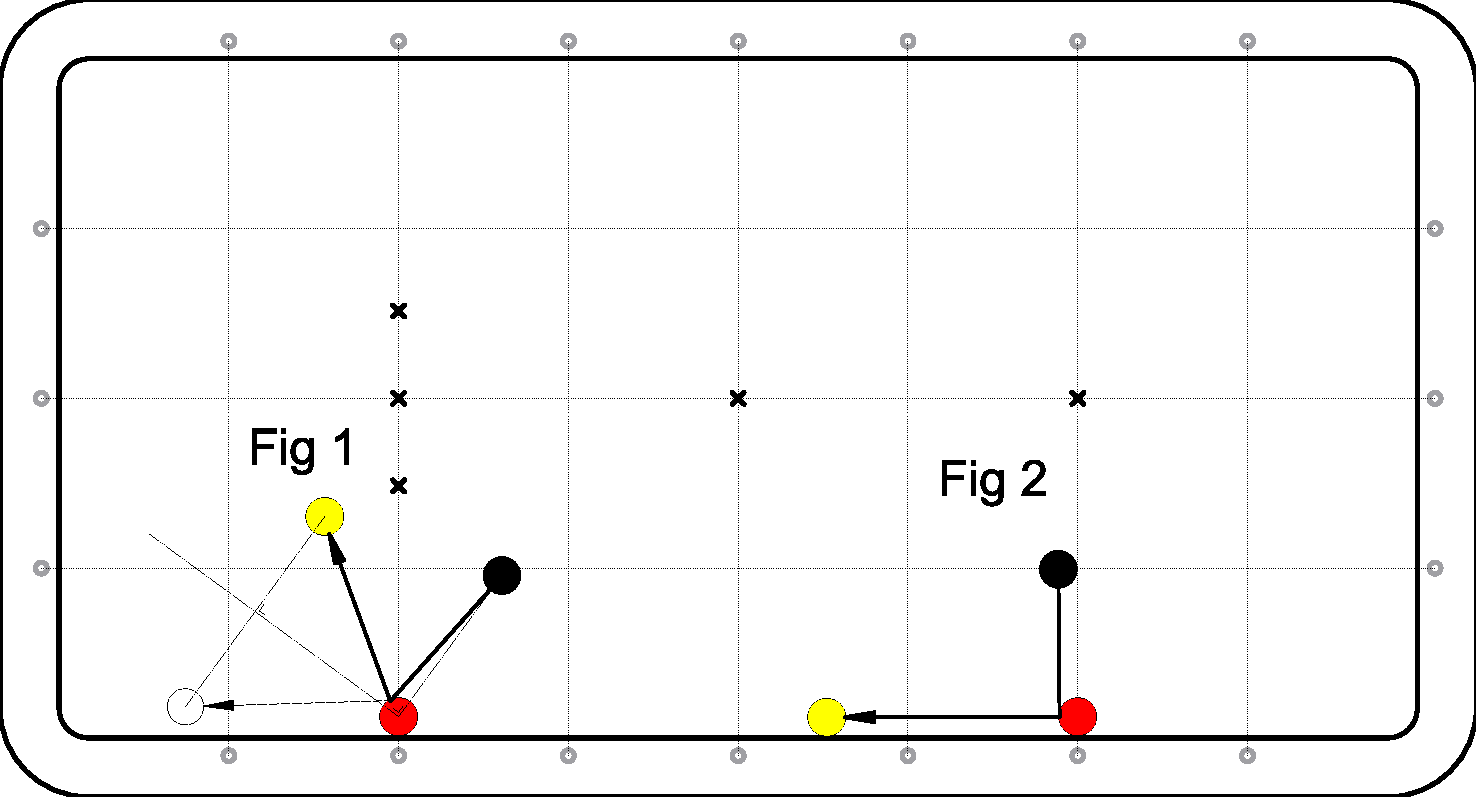
\includegraphics[width=\linewidth]{A/imagesA/A09-01.pdf}
	\caption{Bosse sur la bille colleuse.}
	\label{fig:a09-1}
\end{figure}
\clearpage

%% !TeX spellcheck = fr_FR
% !TeX encoding = ISO-8859-1

\section{Le 1 Bande}

Le 1 bande est un point tr�s fr�quent. Nombreux sont ceux qui se
contentent d'ex�cuter ce point seulement pour ne pas perdre leur tour.
C'est l�, n�gliger la position �ventuellement � exploiter.

En th�orie, il suffit de toucher la 2 de mani�re � percuter la bande au
milieu du segment de bande obtenu en projetant l'image des billes 2 et 3
perpendiculairement sur lui, la 2 et la 3 d�terminant une parall�le �
ladite bande. Si la direction 2-3 n'est pas parall�le � la bande, il
faut s'imaginer le mouvement de � retour � de la 1 pour appliquer une
correction � la th�orie. Avec l'habitude, cette correction � sautera �
aux yeux. Contentons-nous, pour cette premi�re approche, de cas o� les
billes 2 et 3 sont sur une droite parall�le � la bande.

Fig.1 : La distance entre la 2 et la 3 est � peu pr�s le double de la
distance de ces billes � la bande. La th�orie s'applique. Prendre la 2
en demi-bille de mani�re � percuter la bande au milieu du segment comme
d�crit plus haut.

Fig.2 : La distance entre la 2 et la 3 est plus grande que le double de
la distance de ces billes � la bande. La 2 pourrait �tre prise fine mais
il est souvent pr�f�rable de la prendre un peu trop grosse de mani�re �
faire avancer la 2 vers la 3 et de corriger par un bon effet.

Fig.3 : La distance entre la 2 et la 3 est plus petite que le double de
la distance � la bande. En jouant la 2 grosse, on risque que celle-ci
percute la 3 avant l'arriv�e de la 1. Il conviendra de jouer trop fin et
d'apporter une correction par l'effet contraire.

Fig.4 : Cas particulier : la 1 est � bande, et la 2 � une distance
inf�rieure � une bille. Pour une prise en demi-bille jou�e parall�lement
� la bande, appliquons un bon effet pour un angle inf�rieur � 45�, pas
d'effet pour un angle de 45� et effet contraire pour un angle sup�rieur
� 45�. Le r�sultat, en douceur, est surprenant. Si la distance 2-bande
est inf�rieure � une demi-bille sans �tre � masquante �, on peut encore
passer mais prudence : le coup peut se faire masquer par la 2. Si la
distance 2-bande est sup�rieure � une demi-bille, l'effet contraire sera
plus souvent n�cessaire.

Remarque :

\begin{itemize}
	\item
	Le point de base sera rapidement assimil�. L'entra�nement conseill�
	est de s'acharner jusqu'� ce que � chaque r�alisation, les 3 billes
	soient dans un � chapeau �, assurant ainsi la suite de la s�rie...
\end{itemize}

\begin{figure}[htb]
	\centering
	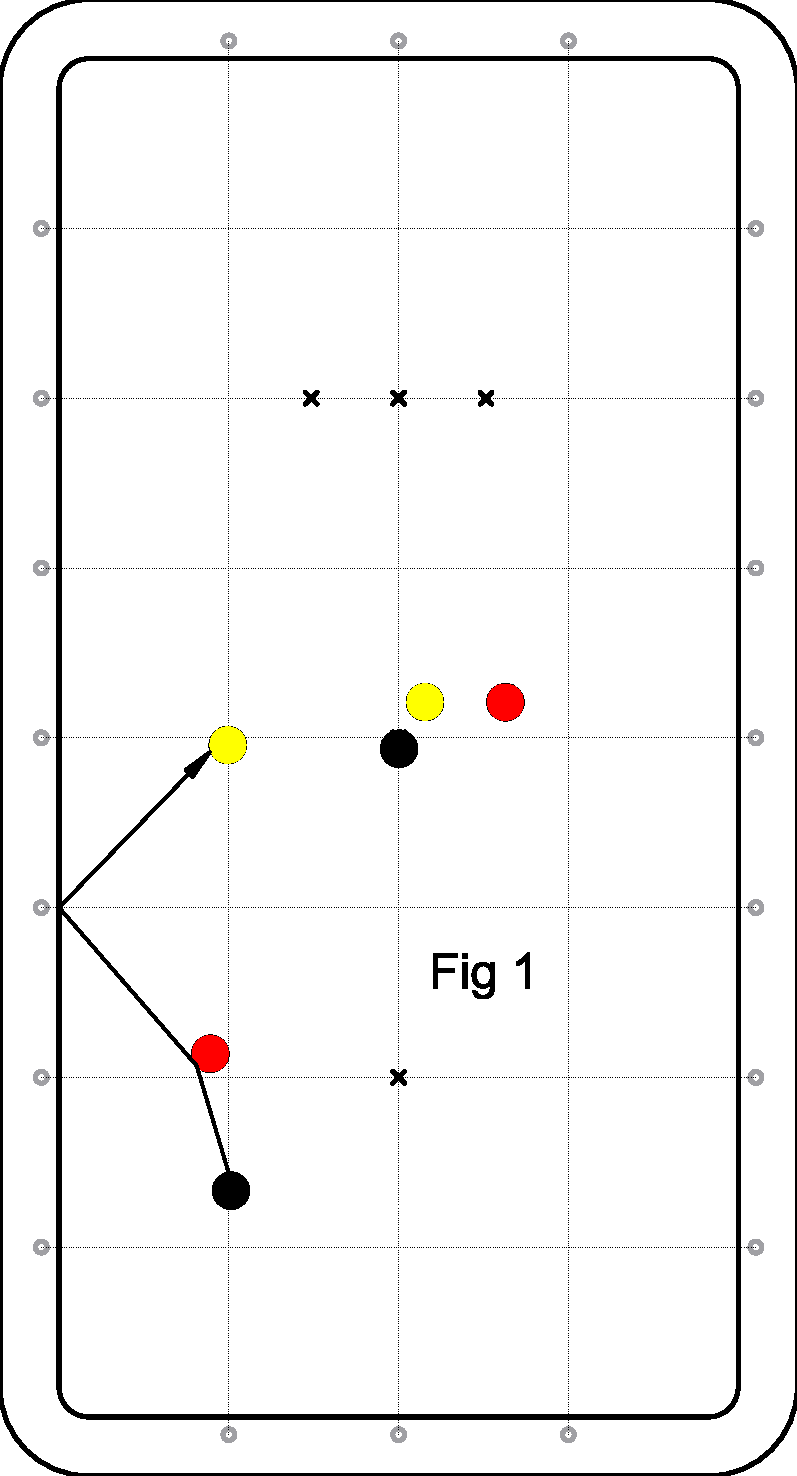
\includegraphics[width=0.85\linewidth]{A/imagesA/A10-01.pdf}
	\caption{Le 1 Bande}
	\label{fig:a10-1}
\end{figure}
\begin{figure}[htb]
	\centering
	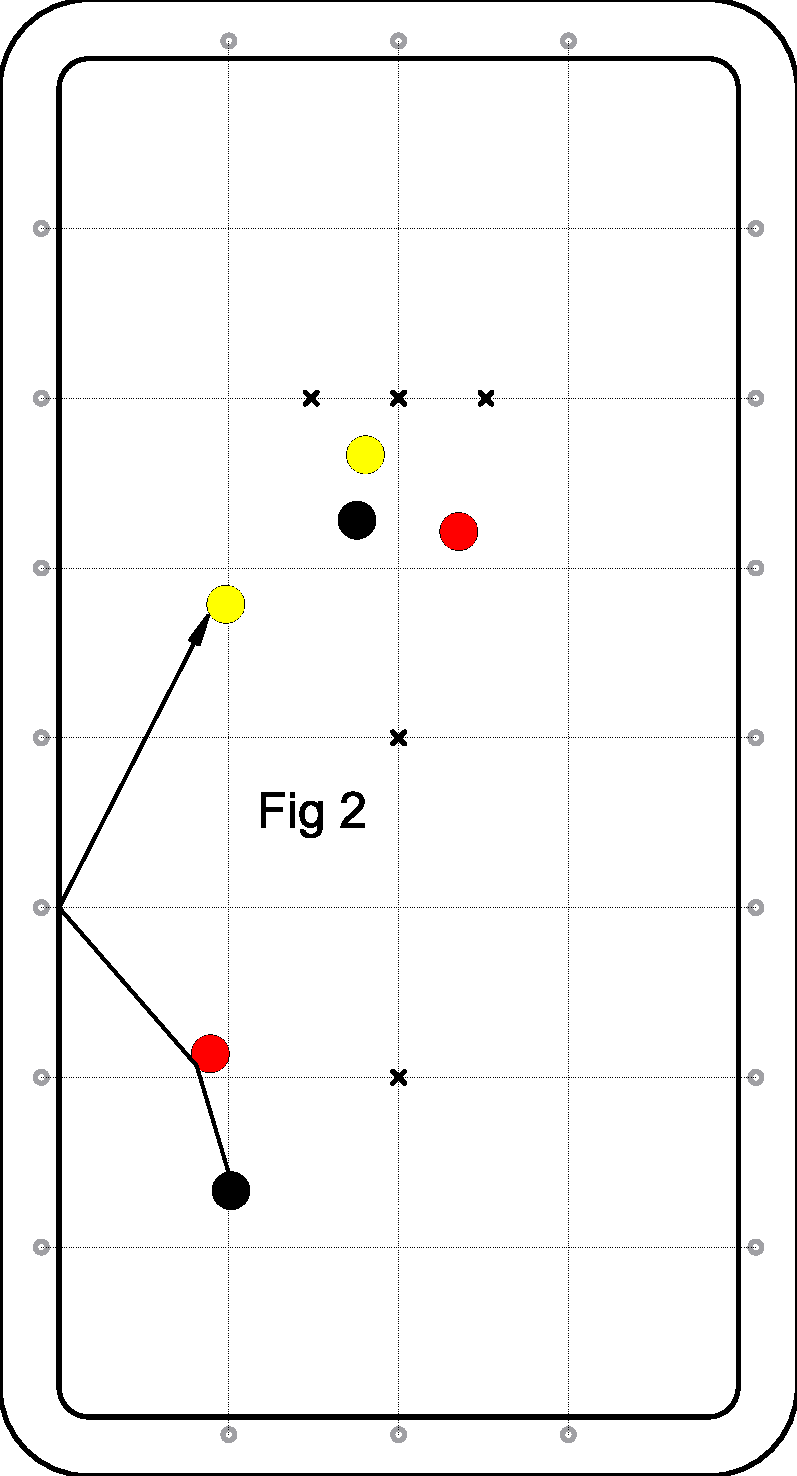
\includegraphics[width=0.85\linewidth]{A/imagesA/A10-02.pdf}
	\caption{Le 1 Bande}
	\label{fig:a10-2}
\end{figure}
\begin{figure}[htb]
	\centering
	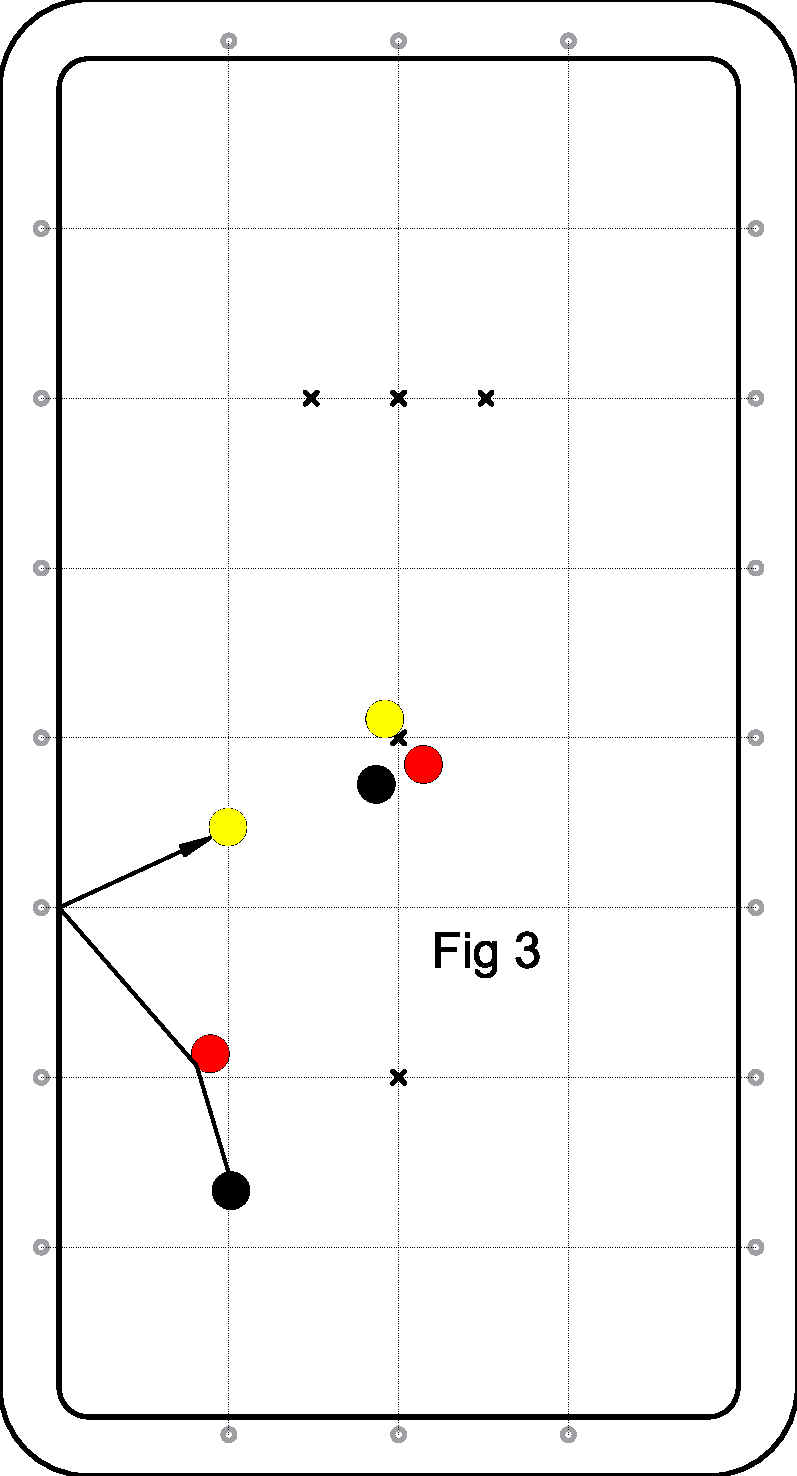
\includegraphics[width=0.85\linewidth]{A/imagesA/A10-03.pdf}
	\caption{Le 1 Bande}
	\label{fig:a10-3}
\end{figure}
\begin{figure}[htb]
	\centering
	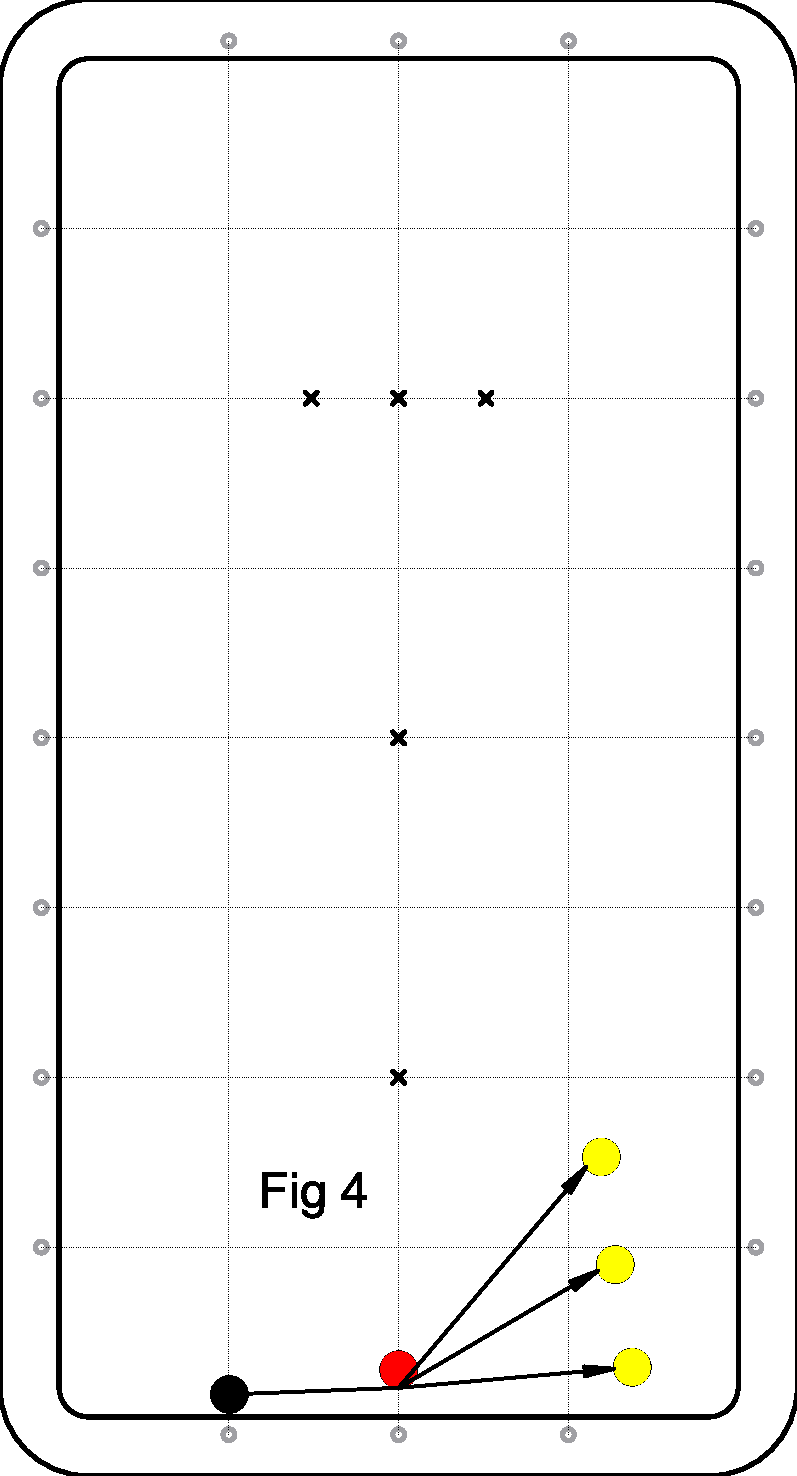
\includegraphics[width=0.85\linewidth]{A/imagesA/A10-04.pdf}
	\caption{Le 1 Bande}
	\label{fig:a10-4}
\end{figure}

\clearpage

%% !TeX spellcheck = fr_FR
% !TeX encoding = ISO-8859-1

\section{2 bandes retour par la bissectrice}

La bissectrice de l'angle de coin offre la particularit� � d'attirer �
les billes en rendant leur mouvement parall�le � elle : ce n'est
�videmment pas vrai ! Il s'agit d'une tendance seulement et dans
certains cas, cette tendance nous sera bien utile. Si une bille roule
parall�lement � la bissectrice, mue d'un effet normal mais favorable,
elle reviendra parall�lement � cette bissectrice, sym�triquement au
premier mouvement (ou presque).

Figure 1 : Cette figure illustre cette particularit�. Bien que lorsque
nous aurons atteint un certain niveau nous n'y penserons plus, il est
int�ressant de s'exercer � ce point. Les billes 2 et 3 sont situ�es sur
des parall�les de chaque c�t� et �quidistantes de la bissectrice.
N'h�sitons pas ! Prenons la 2 de telle sorte que le trajet de la 1 soit
parall�le � la bissectrice et mue d'un effet favorable. La 1 revient par
le coin, parall�le et sym�trique � son premier trajet par rapport � la
bissectrice : le point, d'apparence d�licate, est devenu inratable !

Figure 2 : Ceci illustre seulement une tendance qu'il conviendra de se
rendre famili�re. La 3 est situ�e sur la bissectrice de l'angle de coin
et la 2 pr�s d'une bande (ici la petite mais le probl�me est valable sur
la grande aussi mais la position des billes est alors rarement aussi
int�ressante car la grande bande � �carte le jeu
\textgreater{}\textgreater{} et la petite � ram�ne �). Prendre la 2 en
visant le milieu de la portion de bande entre la 2 et le coin, effet
favorable, haut de bille. Je dis bien viser et pas toucher ! En effet,
vu la dimension de la bille, celle-ci touchera un peu avant le milieu si
le point est court (distance 2-coin courte) et assez bien avant, si le
point est long (distance 2-coin longue).

Remarque :

\begin{itemize}
	\item
	Ce point est plus � � sentir � qu'� calculer.
	\item
	Certains billards allongent et d'autres � cassent �. Il faudra en
	tenir compte.
	\item
	Un effet bas de bille � rabat �. Pour � soulever �, il faut viser la
	bande, plus pr�s de la 2 que du coin, pour rabattre, plus pr�s du
	coin.
	\item
	Attention, si la 2 est �cart�e de la petite bande de plus de dix
	centim�tres environ, il conviendra de viser plus pr�s du coin, etc.
\end{itemize}

Il existe donc beaucoup d'adaptations � ce point qui seront volontiers
propos�es lors de la pr�sentation � sur le terrain �.

\begin{figure}[htb]
	\centering
	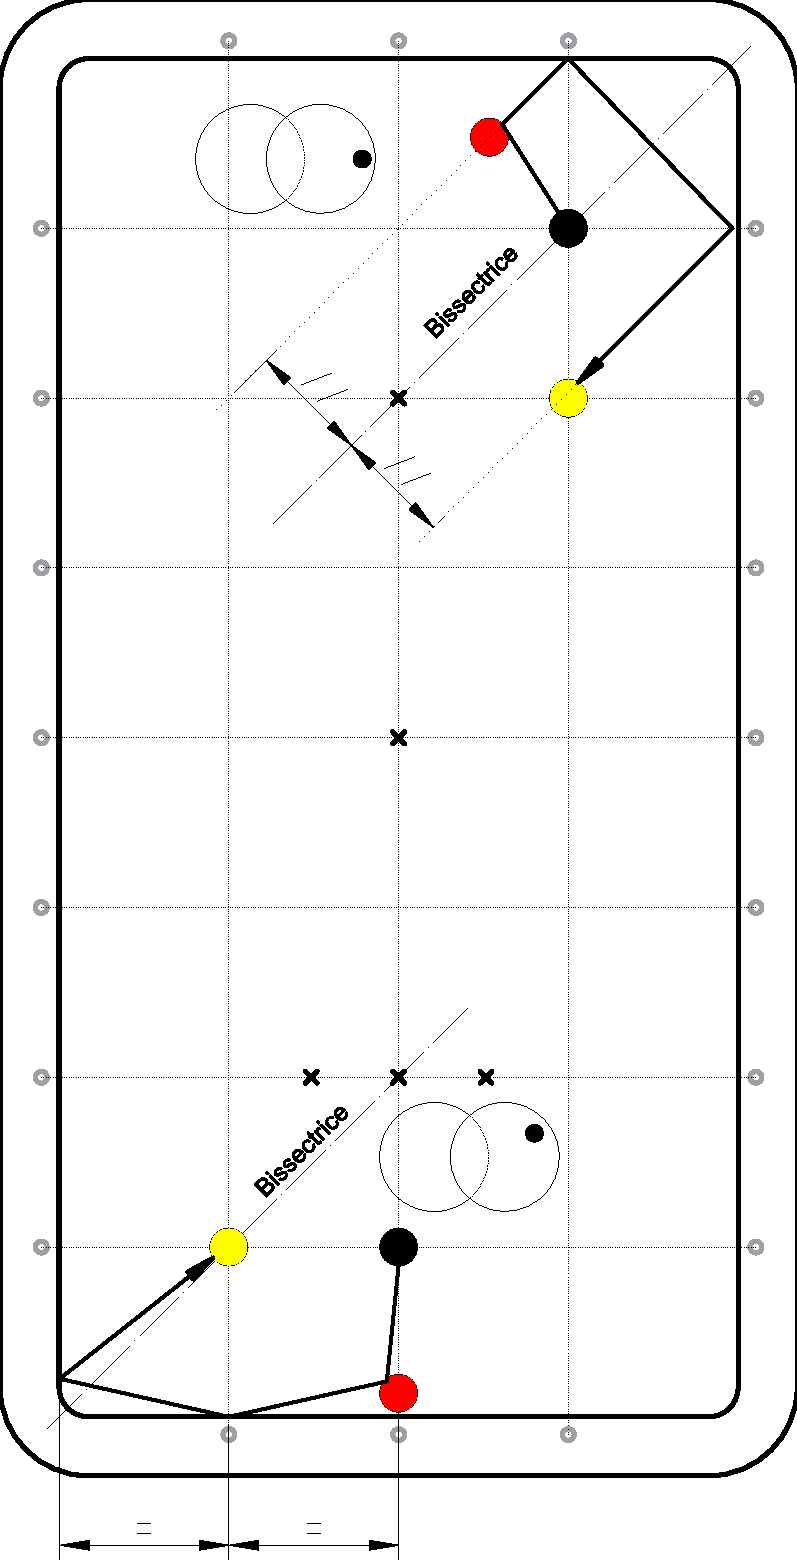
\includegraphics[width=0.85\linewidth]{A/imagesA/A11-01.pdf}
	\caption{2 bandes retour par la bissectrice.}
	\label{fig:a11-1}
\end{figure}
\clearpage

%% !TeX spellcheck = fr_FR
% !TeX encoding = ISO-8859-1

\section{Le	coul�-bande}

Nous avons d�j� vu le coul� simple. Ici, une difficult� suppl�mentaire
appara�t : de par la disposition des billes, la 1 sera emp�ch�e par une
bosse avec la 2.

Figure 1 : Cette figure illustre le cas o� la 2, apr�s le choc d'avec la
1, percute la bande puis vient se mettre dans le chemin de la 2. Une
autre solution devra �tre trouv�e, si possible une finesse, un mass�
(voir 3�ann�e - les planches �C�), un 1 bande sur une autre bande ou
m�me carr�ment une carambole dans les cas les plus difficiles. Cette
solution alternative permet de rester au billard mais donne rarement une
position de \textless{}\textless{} construction �.

Figure 2 : On peut pallier l'inconv�nient du contre en coulant � droit
devant � avec un maximum d'effet contraire par rapport � la 2. Celle-ci,
imprim�e d'un effet contraire, s'�carte de la perpendiculaire � la bande
et �vite la 3 et surtout aussi, la 2 au retour comme l'indique le
pointill�. La 1, maintenant, a le champ libre et fonce sur la bande
droit devant mue d'un effet important (effet toupie), favorable � une
d�viation vers la 3. Les billes 1 et 2 ont donc un mouvement de
d�solidarisation. La 1 reste en position dominante, face aux billes 2 et
3, chass�es du m�me c�t�. Port� moyennement fort, le coup donne
suffisamment d'�nergie pour permettre � la 2 de revenir dans le jeu par
doublage. Ce point demande une bonne pr�cision mais si on joue
absolument droit c�d absolument plein sur la 2 avec le � plein
\textgreater{} effet, la r�ussite est certaine !

Figure 3: Vu la situation, on aurait pu tenter un direct mod�r� ce qui
pourrait donner au coup suivant, un r�tro � rentrant � les billes dans
le � tiers �. Cependant, si on se sent bien,
appliquant un � coul�-bande � comme pour la figure 2, le coup est sans
danger et chasse imm�diatement les billes dans le tiers. Cette solution
donne souvent plus de chance de � serrage � du jeu.

Remarque : si on parvient � couler en � descendant � dans la 1, l'effet
imprim� sera tr�s important et nous permettra de r�aliser des angles
tr�s � �tal�s � au rebond, voire, comme on dit parfois, faire des angles
� impossibles �. Acharnons-nous : la droiture du corps et la position
ferme de la main doivent �tre parfaites...

\begin{figure}[htb]
	\centering
	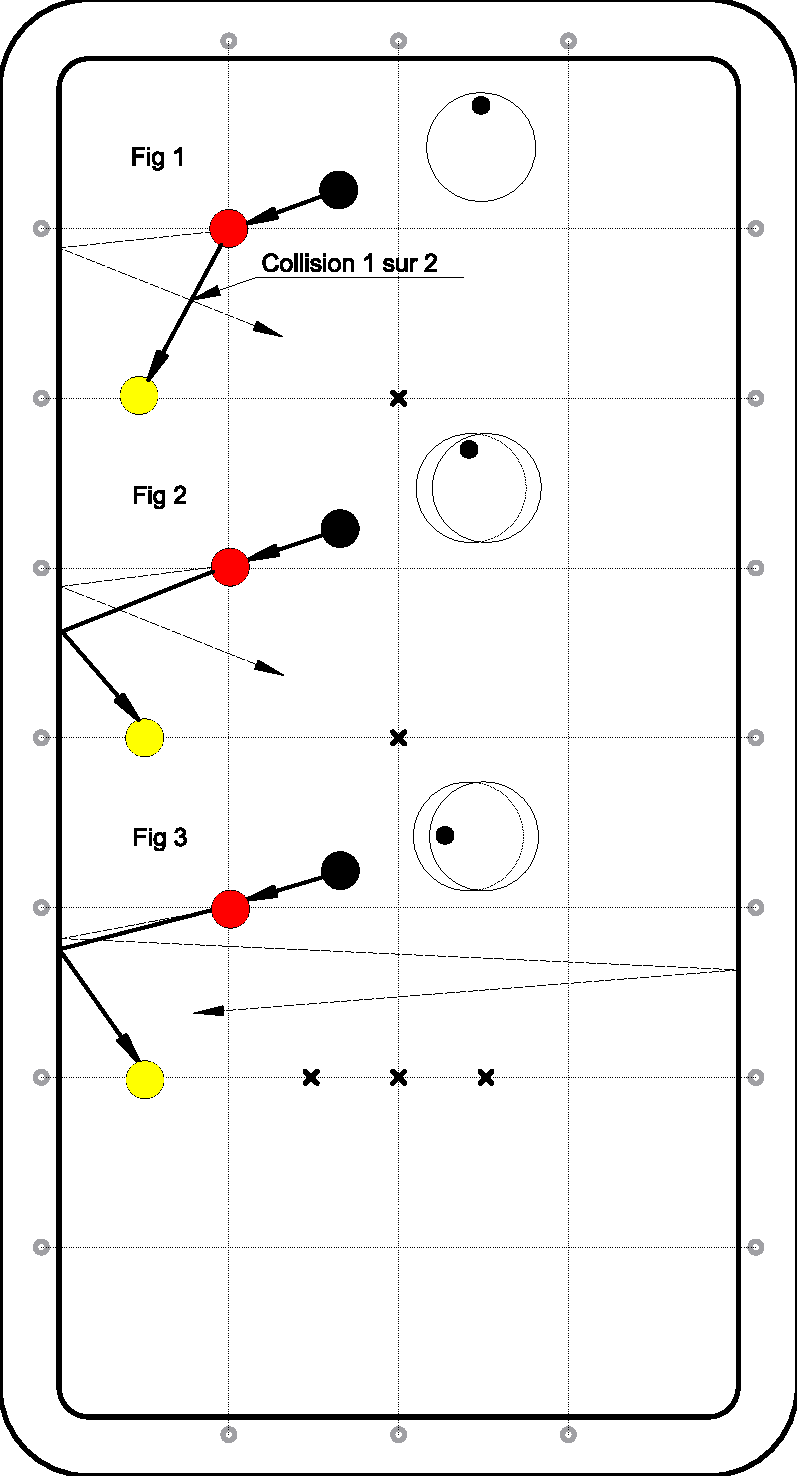
\includegraphics[width=0.85\linewidth]{A/imagesA/A12-01.pdf}
	\caption{}
	\label{fig:a12-1}
\end{figure}
\clearpage

%% !TeX spellcheck = fr_FR
% !TeX encoding = ISO-8859-1

\section{Le coul�-bosse}

Le coul� simple est ais�ment appris, m�me par un d�butant. Le coul�
bande est un peu plus difficile. Le coul� bosse l'est encore davantage.
La � bosse � fait peur. Une fois cette peur vaincue, le point devient
plus facile. Encore une fois, la confiance en soi travaille pour la
r�alisation du point.

Figure 1 : La 2 colle la bande. Viser une moiti� de bille du r�tro (pour
un angle inf�rieur au droit), prise en t�te (haut de bille) et avec
effet contraire maximum. Faisant corps au moment du choc, les billes 1
et 2 se d�tachent ensemble pour venir en jeu serr� � la 3. Une
possibilit� de s�rie s'annonce...

Figure 2 : La 2 ne colle pas. La prise de la 2 est la m�me que celle
pour la figure 1 mais peut-�tre un peu plus grosse, comme si on jouait
pour effleurer l'int�rieur de la 3. La bosse de la 2 en retour sur la 1
repousse celle-ci vers l'ext�rieur de la 3. Ici encore, le jeu se serre
et annonce une s�rie possible...

Figure 3 : On peut r�aliser ce point avec ou sans bosse. Avec bosse,
appliquer un effet inverse au sens du jeu. Le coul� est direct en visant
comme si la 3 se trouvant � devant � elle-m�me. La bosse de la 2 au
retour de la bande sur la 3, pousse la 3 sur la 1, �ventuellement pour
la seconde fois si la 1 avait d�j� percut� la 3. On esp�re que la bosse
de la 3 sur la 1, permet � l'axe 2-3 de ne pas se masquer � la 1 sinon :
c'est la ligne droite : une hantise pour les amateurs de billard. Sans
bosse : mettre l'effet dans le sens du jeu. Cette prise exige une plus
grande pr�cision dans la force � appliquer : la 2 ne rencontrant plus le
barrage au retour, risque de s'�carter loin du jeu ou de rester en de��
et d'offrir encore une fois, trois billes align�es. L'id�al serait que
la 2 vienne � hauteur de la 3 ou s'�carte l�g�rement. En tous cas, il ne
faut pas tenter ce coup pour subir une bosse non d�sir�e, le r�sultat
serait impr�visible.

Figure 4 : C'est une variante de la figure pr�c�dente. Nous ne sommes
plus face � la bande mais bien au coin. La 2 revient par deux bandes
avec des trajectoires parall�les � l'axe. L'effet doit toujours �tre
favorable et la bosse arri�re presque toujours �vit�e.


\begin{figure}[htb]
	\centering
	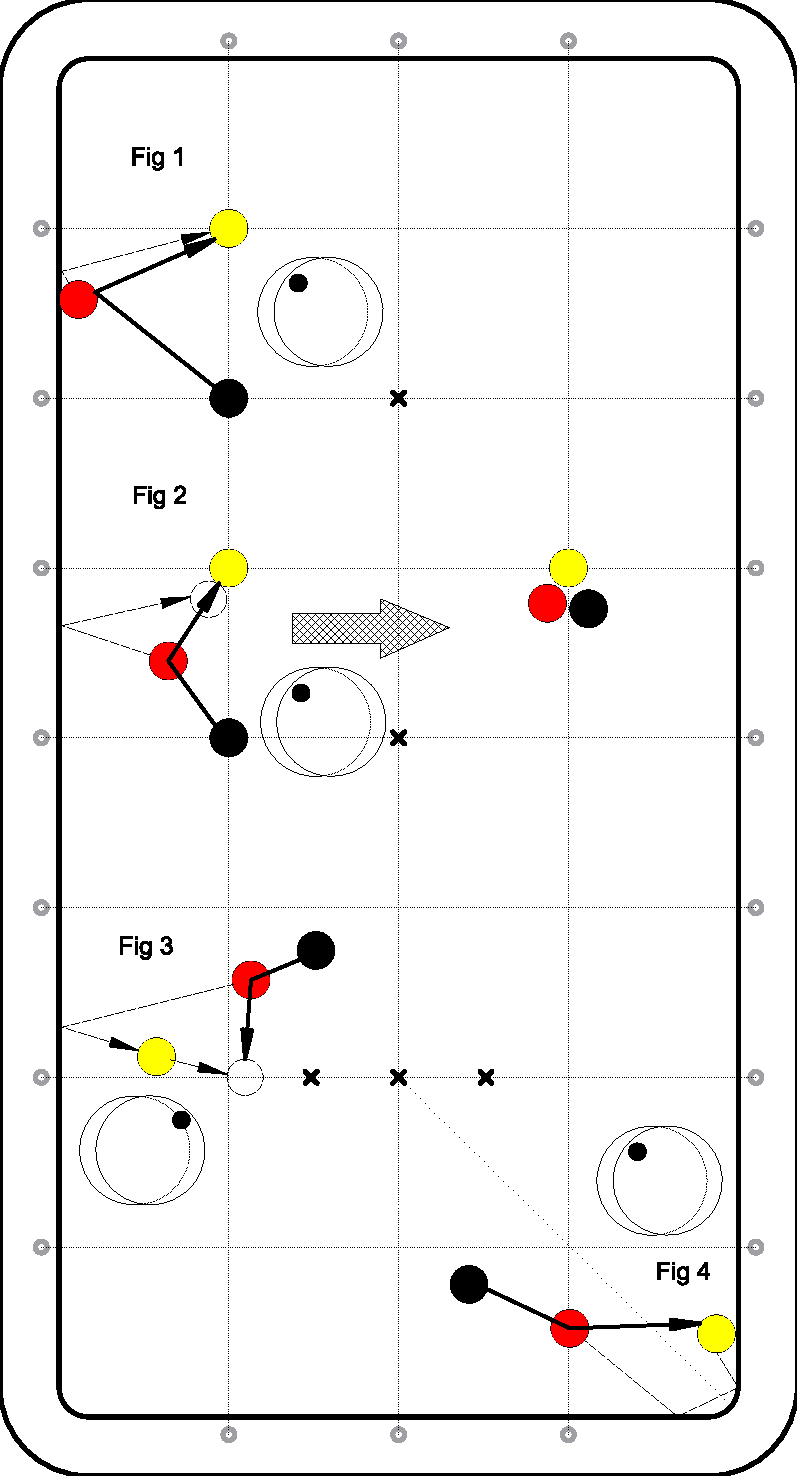
\includegraphics[width=0.85\linewidth]{A/imagesA/A13-01.pdf}
	\caption{Le coul�-bosse}
	\label{fig:a13-1}
\end{figure}
\clearpage

%% !TeX spellcheck = fr_FR
% !TeX encoding = ISO-8859-1

\section{Le r�tro-bande}

Une fois la technique du r�tro bien en main, on s'habituera facilement �
ce coup. Le ramen� ou rappel est plus ou moins s�r. Cependant, l� o� le
r�tro direct ne ram�ne pas directement, il est parfois possible de
s'assurer une rentr�e convenable en s'aidant de la bande, se figurant
une bille 3 virtuelle plac�e de l'autre c�t� de la bande qui lui est
proche sym�triquement � la 3 r�elle (donc en dehors de la table). En
voici deux exemples :

Figure 1 : Le r�tro direct est une solution mais il entra�ne la 2 hors
de la rentr�e. La 2 toucherait la petite bande trop loin du coin oppos�
et elle s'�carterait irr�m�diablement. Pour minimiser cet �cart :
prendre la 2 en r�tro de pr�f�rence basse, effet droit si la direction
1-2 est loin du coin et effet gauche si la direction 1-2 est trop pr�s
du coin et jouez comme si la 3 �tait situ�e sym�triquement de l'autre
c�t� de la bande qui lui est proche (3'). Id�alement, la 2 tournera via
la petite bande sup�rieure, la grande bande oppos�e, la petite bande
inf�rieure, la grande bande proche et vient s'arr�ter dans le barrage
form� par la 1 et la 3.

Figure 2 : Ce point est tout en d�licatesse. Un r�tro simple ferait
d'abord toucher la petite bande � la 2 qui ne pourrait plus rentrer. Si
la direction 1-2 coupe la petite bande mais tr�s � haut �, on peut
encore jouer r�tro direct avec effet ras du tapis maximum et contraire :
la 2 ne s'�cartera pas ou peu. Si la direction 1-2 coupe trop bas ou
bien trop haut sur la grande bande (� appr�cier), il est encore possible
de serrer le jeu en appliquant un r�tro bande effet contraire maximum.
En restant pr�s de la 3, la 1 constitue un barrage au retour de la 2.

Remarque : Ces deux exemples montrent des applications assez simples du
r�tro. Cependant, il ne faut pas s'y tromper et restons prudents. Ils
demandent un s�rieux entra�nement avant d'�tre poss�d�s, non seulement
pour la pr�cision du coup mais aussi et surtout pour la force n�cessaire

\begin{figure}[htb]
	\centering
	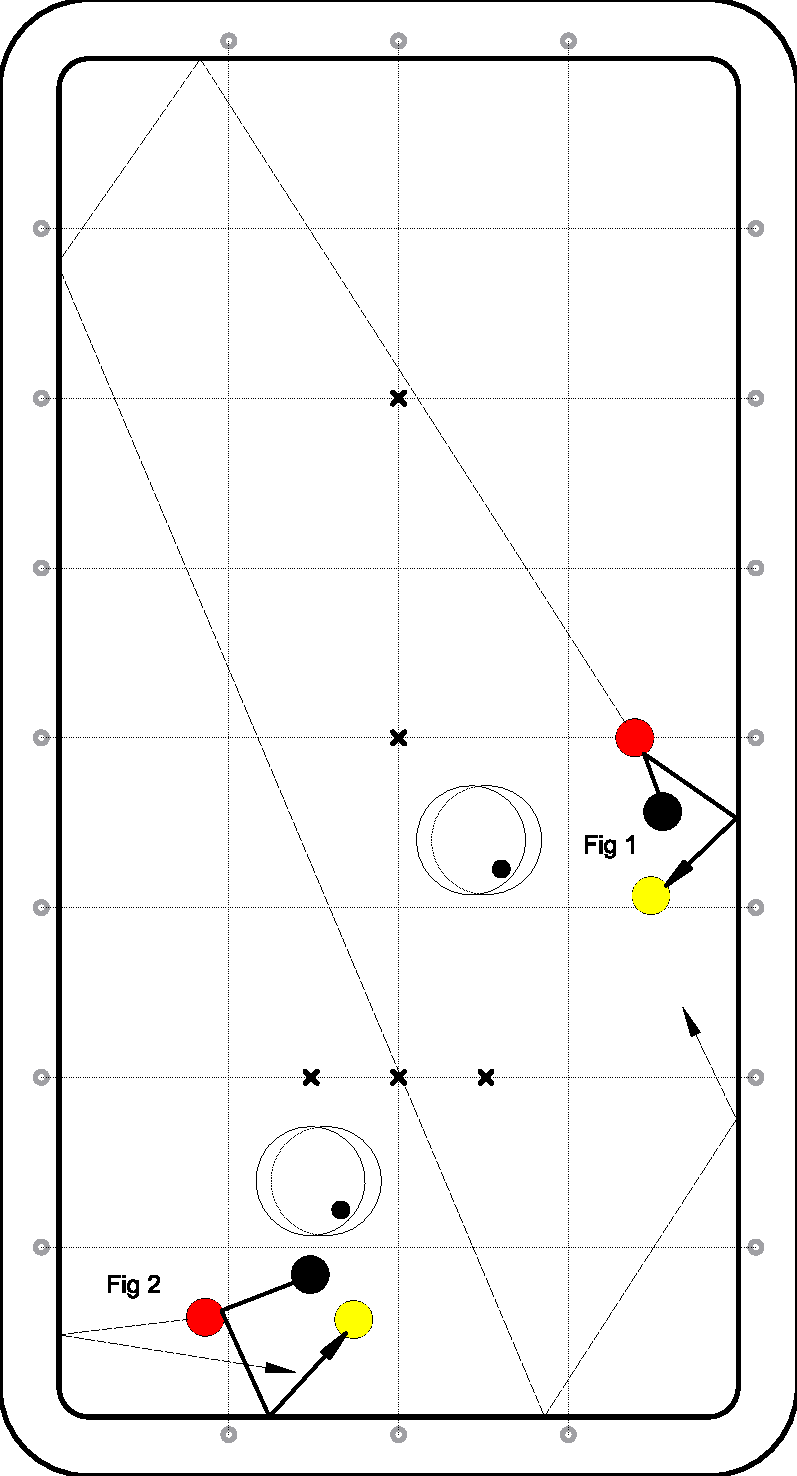
\includegraphics[width=0.85\linewidth]{A/imagesA/A14-01.pdf}
	\caption{Le r�tro-bande}
	\label{fig:a14-1}
\end{figure}
\clearpage

%% !TeX spellcheck = fr_FR
% !TeX encoding = ISO-8859-1

\section{Le petit coul�}

Sans trop de danger, le petit coul� est possible jusqu'� une distance de
1 centim�tre entre les billes 1 et 2. Il demande une grande souplesse,
de la prudence et de la d�licatesse. A une distance plus courte, le
queut� est dangereux, c�d que la canne, selon la th�orie, serait encore
en contact de la 1 lorsque cette derni�re percuterait la 2 ce qui
constitue la d�finition officielle du queut�.

Bien que cette th�orie soit exacte, en pratique, la v�rit� est souvent
diff�rente. En fait, pour ex�cuter un coul�, il faut allonger, c�d
accompagner la 1 dans son mouvement. Fort bien, mais accompagner ne
signifie pas rester en contact sinon le proc�d� a frott�, la bille a
roul� en se frottant : c'est une faute qui est visible lorsque la fl�che
� roule � sur la bille. En r�alit�, le proc�d� reste en contact tr�s peu
de temps. La 1 subit une acc�l�ration qui la d�tache directement du
proc�d� mais subit un ralentissement au choc avec la 2 avant d'acc�l�rer
� nouveau sous l'impulsion de l'effet longitudinal produit par
l'accompagnement de la canne. C'est ce ralentissement qui fait danger
car la canne dans son mouvement avance encore... et risque de rattraper
la 2 � ce moment : queut� ! Ce queut� est facile � d�pister pour
l'arbitre car les billes 2 et 3 auront tendance � se mouvoir en m�me
temps et � la m�me vitesse. Les � anciens \textgreater{}\textgreater{}
appellent cette faute : � une charrette �. L'arbitre, bien plac� sur le
c�t� de la direction des billes doit annoncer � faute � et passer la
main � l'autre joueur.

Le point se joue comme un coul� traditionnel, canne horizontale,
mouvement l�ger et prolongeant en veillant � retenir la canne avant que
la 1 ne percute la 2. Si la distance est vraiment trop courte, on peut
relever l�g�rement la fl�che d�s le coup port�. Cela rassure sur la
validit� du point mais plus tard, il sera pr�f�rable de ne pas le faire
pour une meilleure ma�trise du jeu serr�. Ce point fait peur. Beaucoup
lui pr�f�re un mass�.

Comme entra�nement, je conseillerais de placer les billes 1 et 2 � 5 cm.
l'une de l'autre et de r�aliser le coul� en rassemblant les 3 billes
dans un � chapeau � (les 3 billes doivent pouvoir �tre couverte par une
main ouverte). Ex�cuter des s�ries de 10 essais jusqu'� une s�rie
r�alis�e � 100\% de r�ussite (!). Ensuite placer les billes 1 et 2 � une
distance de 4 cm. Recommencer les s�ries. Puis placer les billes � 3 cm.
2 et enfin 1 cm.

C'est fastidieux... mais ce sera payant. Il conviendra de s'armer de
patience et d'obstination. Il faut prendre le temps n�cessaire de bien
poss�der cette �tape.

\begin{figure}[htb]
	\centering
	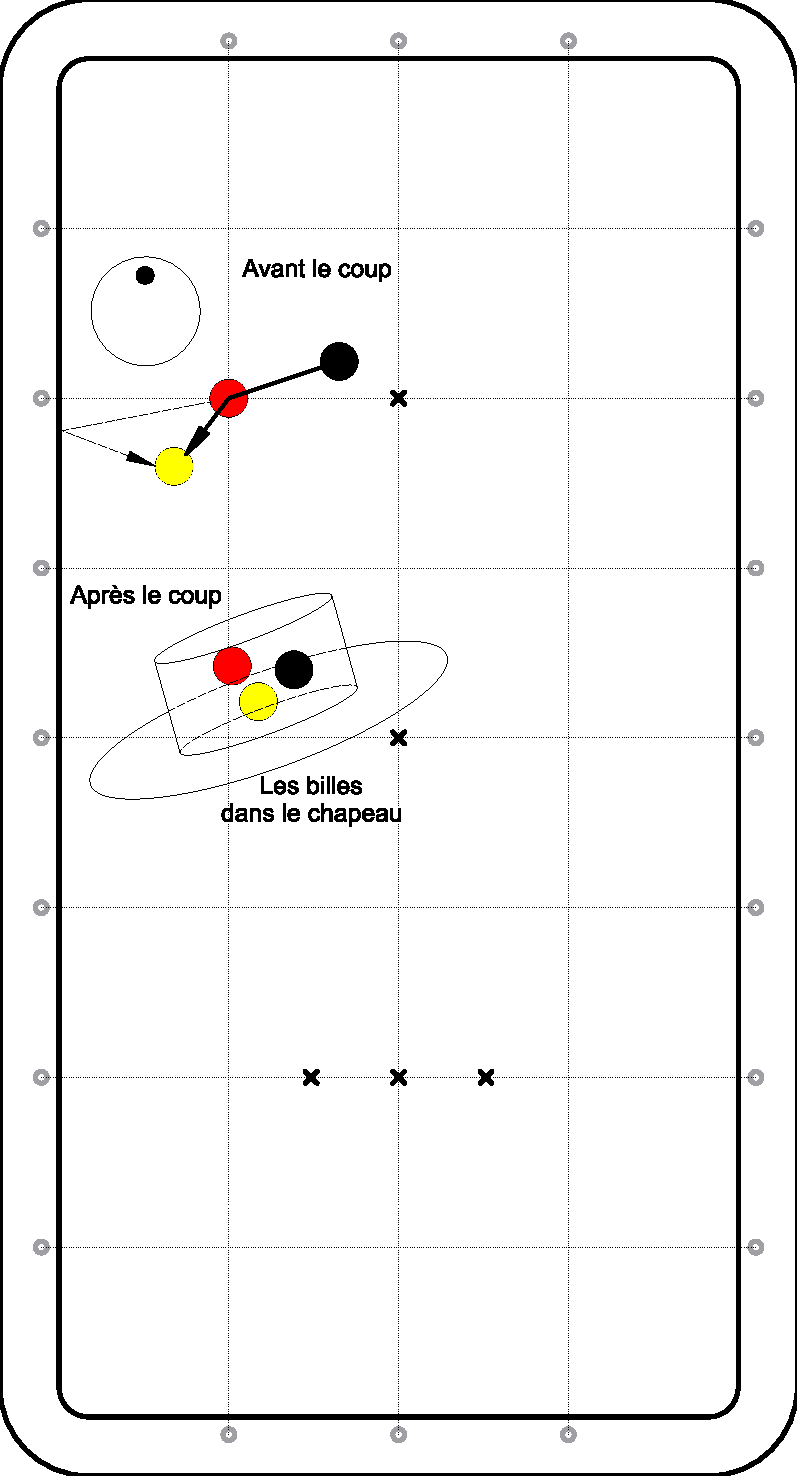
\includegraphics[width=0.85\linewidth]{A/imagesA/A15-01.pdf}
	\caption{Le petit coul�}
	\label{fig:a15-1}
\end{figure}
\clearpage

%% !TeX spellcheck = fr_FR
% !TeX encoding = ISO-8859-1

\section{Le petit r�tro}

Le petit r�tro est un point d'une d�licatesse et d'une souplesse de
toute premi�re importance pour la construction des s�ries. Plus tard,
par la justesse du coup, il permettra de bien ma�triser le retour de la
2 � dans le paquet � et le maintien du � serrage �. Il est surtout �
employer lorsque les billes sont proches l'une de l'autre.

Les billes sont � ce point rapproch�es qu'on pourrait jouer fin ou gros,
le point est inratable. Il serait r�ussi mais pas pour autant, bien
choisi. En effet, du choix d�pendra la suite de la s�rie. La position de
la 2 est � soigner particuli�rement.

Figure 1 : pour l'entra�nement, nous placerons les billes 1 et 2 �
environ 5 cm. l'une de l'autre. Nous ex�cuterons le r�tro de mani�re que
la 2 revienne dans le � chapeau �. Quand nous aurons r�ussi 10 fois de
suite, placer les billes 1 et 2 � 4 cm. d'intervalle. Recommencez la
m�me s�rie d'essais puis placez les billes 1 et 2 � 3, � 2 et enfin � 1
cm d'�cart. Pour cet exercice, la main arri�re doit se rapprocher du
point de d�s�quilibre de la canne sans la presser. Nous veillerons �
appliquer �ventuellement un effet pour assurer le retour de la 2 dans le
paquet. Une fois cet �puisant exercice r�ussi � 100 \% (!), passez � la
figure 2.

Figure 2 : Les billes sont proches de la bande, la 2 en �tant la plus
proche. Appliquez le r�sultat de votre pr�c�dent exercice et veillez �
ce que la 2 revienne en percutant doucement la 1 qui fait barrage : sans
le savoir, vous venez d�j� de toucher aux pr�mices de la s�rie dite � �
l'Am�ricaine �.

Pour affiner votre coup, prendre la 2 la plus grosse possible tout en
veillant � la r�alisation du point, appliquer l'effet qui assure le
retour de la 2 vers la 1 en barrage (bon effet si la 2 est trop avanc�e,
contraire si la 2 est en retard). La main arri�re doit �tre rapproch�e
jusqu'au point de rupture de l'�quilibre de la canne. Ne pas jouer fort
mais souplement.

Remarque : ce point para�t facile. Qu'on ne s'y trompe pas, il ne l'est
pas. De sa bonne ex�cution d�pend la s�rie. Il est vraiment une des
bases de la s�rie am�ricaine, grande ennemie du manque de souplesse.
Attention ! On perd souvent la position pour avoir jou� trop fin !

\begin{figure}[htb]
	\centering
	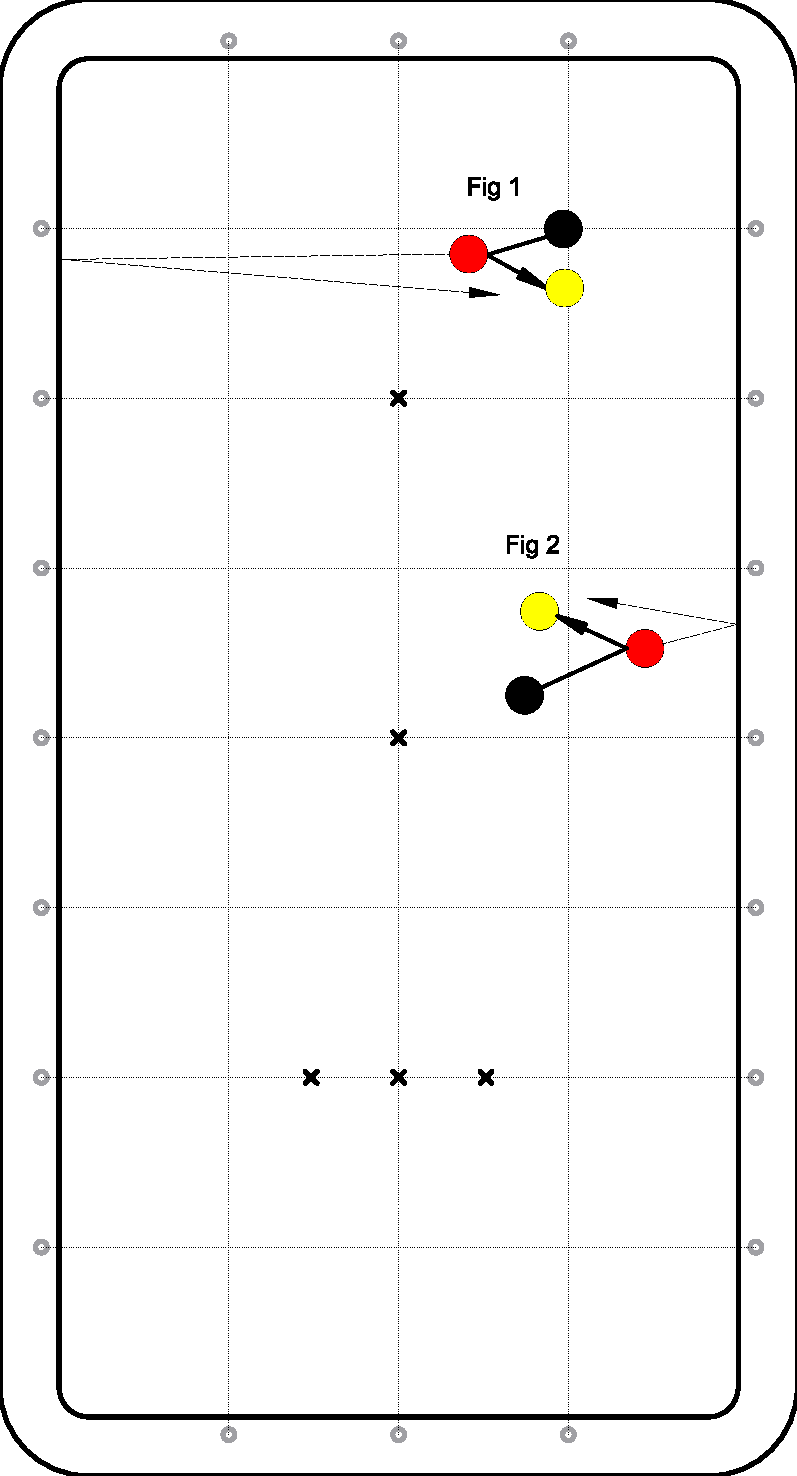
\includegraphics[width=0.85\linewidth]{A/imagesA/A16-01.pdf}
	\caption{Le petit r�tro}
	\label{fig:a16-1}
\end{figure}
\clearpage

%% !TeX spellcheck = fr_FR
% !TeX encoding = ISO-8859-1

\section{Le trois bandes naturel}

Le 3 bandes naturel est ais� de conception et ram�ne le jeu dans le
coin. Les � vrais � joueurs de 3 bandes vous expliqueront qu'il faut
calculer les � mouches � (points de partage dessin�s sur les bandes de
la table) et jouer pr�cis�ment sur celles-ci si on veut faire le point.
Attention, ici nous parlons du jeu de libre ! Si le calcul des �
troisbandistes � (joueurs sp�cialis�s au jeu de 3 bandes) est exact, il
ne nous int�resse ici que tr�s secondairement et de toute fa�on, il est
beaucoup trop t�t pour s'y int�resser. Nous allons tenter de r�aliser en
ramenant la 2 dans le coin. Il y aura un risque de contre, cons�quence
de ce ramen�.

Comme pr�sent� sur la figure, on prend la 2 en demi-bille, coup prolong�
mais pas trop fort, l�ger effet favorable sur la premi�re bande. La
force du coup doit assurer le chemin, sans plus ! Parfois, on peut
affiner le point par une prise un peu plus grosse, de mani�re �
entra�ner la 2 � la suite de la 1, quitte � corriger la trajectoire de
la 1 par un effet un peu plus soutenu. Variante : prendre la 2 par la
gauche en deux tiers coul�s, effet haut �ventuel � gauche. Attention,
cette m�thode est souvent mal appliqu�e ; la 2 prise trop fine, reste en
� chemin �. D'une mani�re g�n�rale mais non exclusive, si la 1 est plus
proche ou �galement proche de la bande voisine que la 2, on pr�f�rera
tenter le 3B (3 bandes) dit naturel. Si la 1 est � �gale distance ou
bien plus �loign�e de la bande proche que la 2, on choisira de
pr�f�rence le 2B par l'avant (ici par la gauche).

Remarque : le contre de la 2 sur la 1 guette. Il suffira de jouer un peu
plus gros avec effet compensatoire ou bien un peu coul� pour l'�viter.

Entra�nement : placer les billes comme sur la figure, la 1 en face de la
troisi�me mouche en comptant � partir du coin sup�rieur (la partie
sup�rieure de la table est la partie la plus �loign�e du joueur lui-m�me
plac� sur un petit c�t�. Selon la position du joueur, le haut et le bas
de la table s'inversent). Placer la 1 en face de la premi�re mouche, �
partir du bas. La 3 est dans le coin. La 1 et la 2 � 30 cm. de la grande
bande. Ex�cuter donc ce point avec un taux de r�ussite d'au moins 70\%
la 2. Ensuite, faites varier la position de la 2, face aux trois mouches
sup�rieures, hormis le coin, puis faites varier la position de la 1 en
la pla�ant � 25cm. ou � 35 cm. de la grande bande.

En avant pour des s�ries d'essais ! Fameux entra�nement que celui-l�.
C'est tr�s fatigant... et amusant car les billes \textless{}\textless{}
voyagent �.


\begin{figure}[htb]
	\centering
	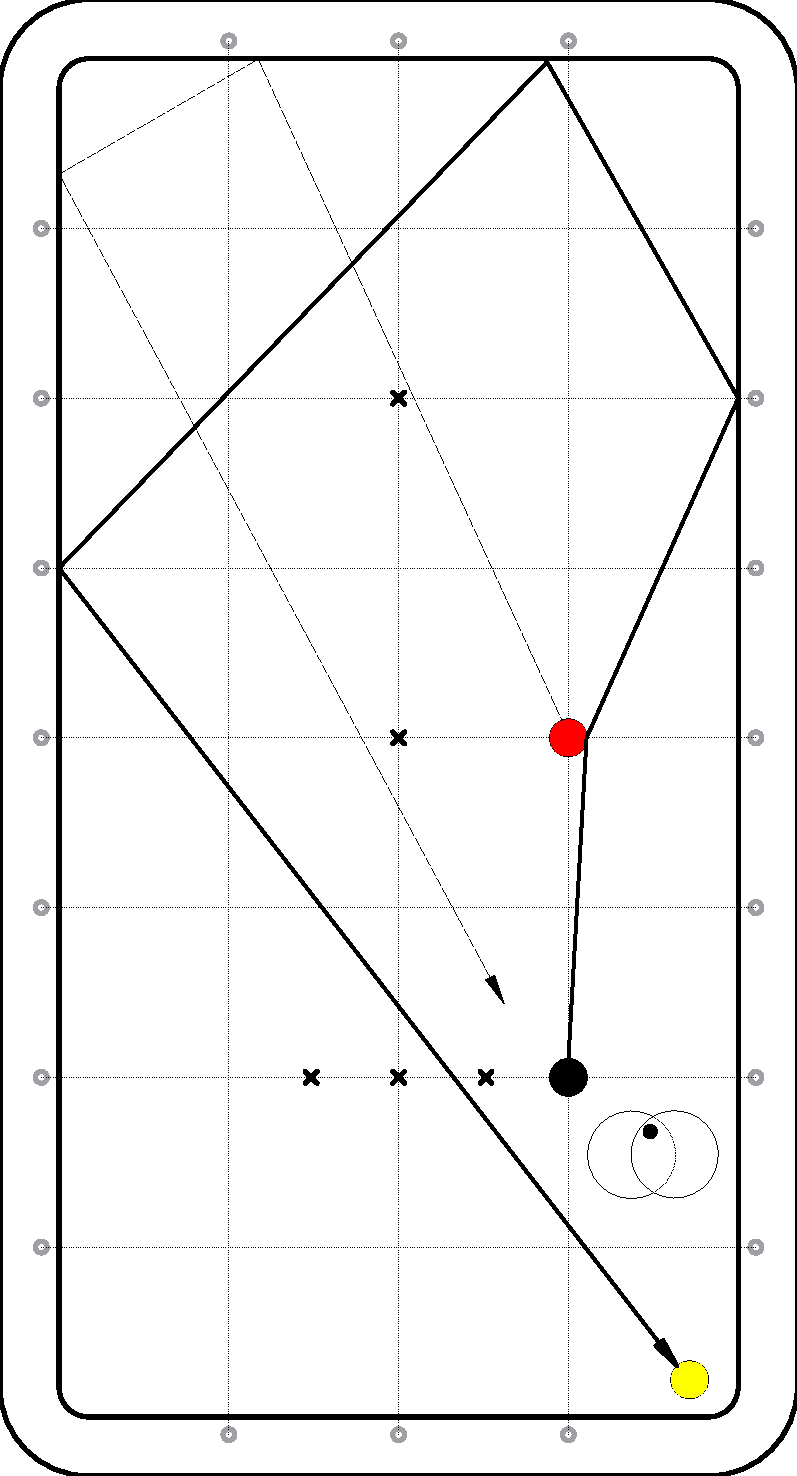
\includegraphics[width=0.85\linewidth]{A/imagesA/A17-01.pdf}
	\caption{Le trois bandes naturel}
	\label{fig:a17-1}
\end{figure}
\clearpage

%% !TeX spellcheck = fr_FR
% !TeX encoding = ISO-8859-1

\section{R�tro Bille-Bande naturel}

Cette position est tr�s fr�quente. Elle permet souvent de ramener la 2
dans � le tiers � et m�me dans le � chapeau �.

Figure : imaginons une bille virtuelle 3' plac�e � l'ext�rieur de la
table sym�triquement oppos�e � son homologue, la bille 3 par rapport �
la grande bande proche. Ne pensons plus � la 3. Consid�rons maintenant
les billes 1, 2 et 3'. Appliquons un r�tro direct. La 1 est jou�e basse
mais pas trop, de mani�re � donner une bonne �nergie � la 2 qui doit
faire le tour de la table alors que la 1 doit s'arr�ter � la 3! On peut
mettre un effet � gauche pour assurer le retour de la 1. La bande coupe
le retour de la 1 pour la d�vier de sa trajectoire de la 3' vers la 3.
L'effet, plus ou moins appliqu�, peut obliger � viser plut�t le dessus
de la 3'. L'application de l'effet bon ou contraire sera fonction de
l'angle 1-2 / grande bande. La principale difficult� sera la force de la
frappe permettant de ramener la 2 dans, un chapeau, aux environs de la
3.

L'angle 1-2 / grande bande doit �tre appr�ci� avant l'essai. Quelques
exemples : a - L'angle en question pr�sent� sur la figure est id�al.
Prise basse en trois quarts, peut-�tre un l�ger effet favorable. Le coup
est moyen et de force moyenne. Cette position est la plus favorable. Ce
n'est pas toujours le cas.

b- L'angle est assez faible (moins de 309). Appliquez un r�tro direct.
La 2 revient en 3 bandes ou 4.

c - L'angle est encore plus petit (10o...). Appliquez un r�tro bande,
effet contraire. La 2 revient en une bande voire deux en s'�cartant un
peu de la grande bande mais pas trop.

d - L'angle est encore plus petit, voire presque nul. Ce sera � voir sur
place. Selon le cas, on appliquera le c - ou bien un r�tro direct,
toujours effet contraire qui permettra � la 2 de peu s'�loigner de la
grande bande au retour.

e - Cas sp�cial : l'angle est trop grand, trop large... et apparemment
ne permet plus de faire tourner la 2. Attention � bien interpr�ter ce
cas sp�cial. La 2 va toucher la grande bande oppos�e avant la petite
bande sup�rieure, nous le � sentons �.

Deux solutions :

\begin{itemize}
	\item
	Appliquer un r�tro direct sur la 3. Le jeu n'est plus ramen� mais les
	billes sont devant nous et permettent d'envisager � nouveau une
	construction de l'autre c�t� de la table.
	\item
	Tentons le diable en appliquant un r�tro bande comme dans le cas
	g�n�ral mais assez haut sur la 1, en dessous du milieu de la bille
	parce qu'il s'agit d'un r�tro et assez haut pour emp�cher une trop
	grande vitesse de la 1 au retour. La 2 est percut�e assez violemment,
	prend le coin sup�rieur en effet contraire et revient dans le chapeau
	! (Pas facile)
\end{itemize}

Entra�nement :

\begin{itemize}
	\item
	Tenter chaque cas des exemples : 100 \% pour le cas g�n�ral, 90\% pour
	les autres.
	\item
	L'exemple e : regardons-le comme un cas singulier mais tout de m�me :
	essayons...
\end{itemize}

\begin{figure}[htb]
	\centering
	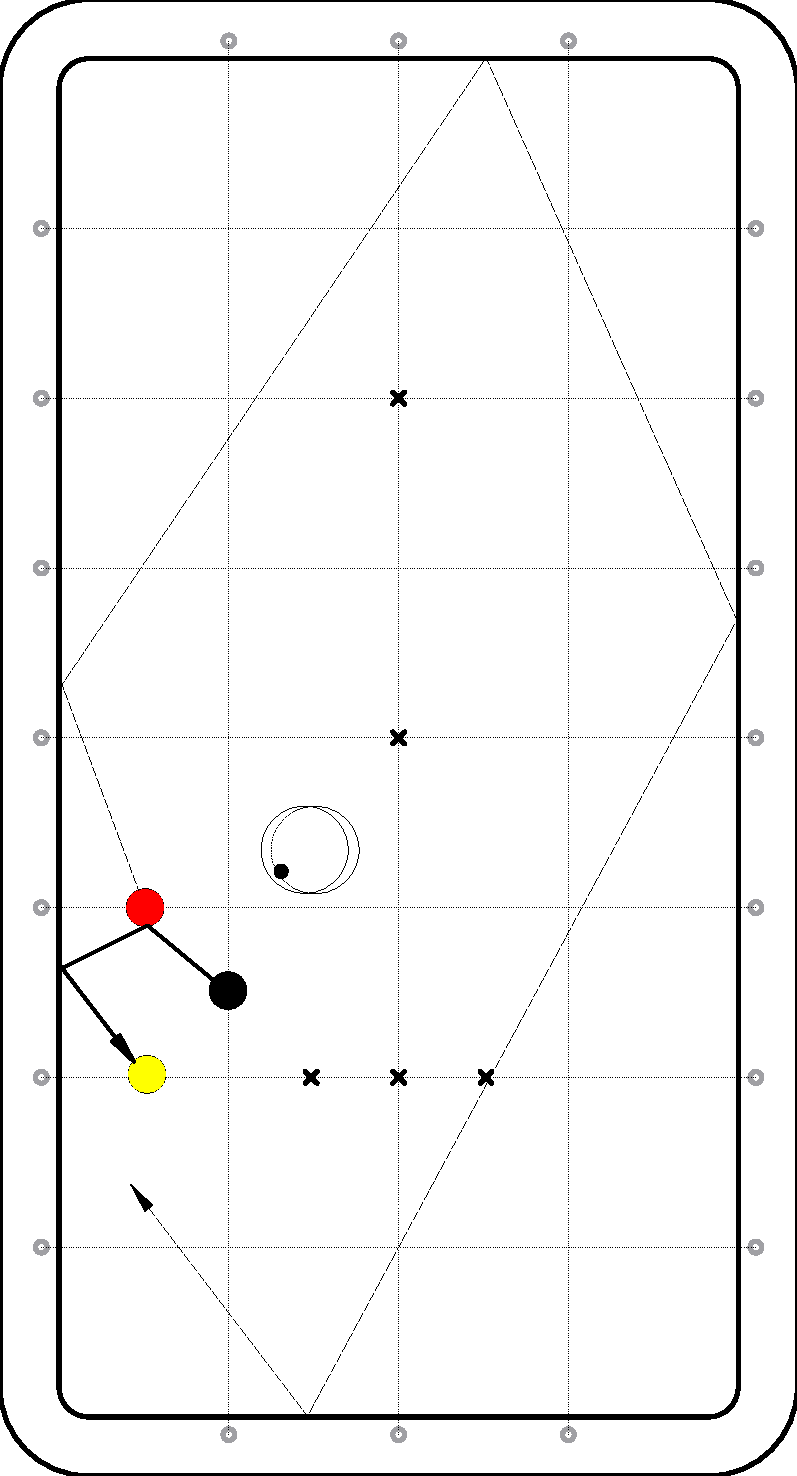
\includegraphics[width=0.85\linewidth]{A/imagesA/A18-01.pdf}
	\caption{R�tro Bille-Bande naturel}
	\label{fig:a18-1}
\end{figure}
\clearpage

%% !TeX spellcheck = fr_FR
% !TeX encoding = ISO-8859-1

\section{Le Carrousel}

Le carrousel est un point assez facile. Il est aussi appel� le �
tourniquet �. La principale difficult� est de faire rouler la 1 afin
qu'elle tourne sans effort. Ce n'est pas si facile... Il conviendra de �
limer � c�d de pr�parer le coup en faisant glisser la canne d'avant en
arri�re et d'arri�re en avant de mani�re absolument r�guli�re, sans
�-coup, non seulement d'une compl�te rectitude mais aussi avec un
abandon total de sa personne. Cela signifie que le joueur doit
s'abandonner � son mat�riel, lui faire confiance. Au dernier limage, le
coup est port� avec la m�me fluidit� qu'au limage, un simple
prolongement au dernier moment. Si nous r�ussissons ce � ne rien mettre
d'autre dans sa canne �, la 1 va rouler avec une fluidit� et une
r�gularit� qui vont jusqu'� lui assurer une plus grande distance
parcourue... et avec une chance accrue d'�viter le contre.

La figure : au niveau de la mouche �c �, prendre la bille en demi, un
peu d'effet � droite et haut de bille. Si on a le contre, jouer un rien
plus fin, ou un rien plus d'effet ou .... Et c'est souvent l� qu'il faut
regarder : voyez la fluidit� du coup port�. On veillera � v�rifier que
la 2 rentre bien dans le coin avec la 3. Remarque : le contre est moins
dangereux si on r�alise le point en 3B s�ches, c�d toucher la 3 par
devant.

Variantes : Plus la 2 est dans le � bas � de la table, plus on �
grossira � la prise. Ainsi face � la mouche � d �, prendre une bonne
demi-bille, face � e, prendre six dixi�mes et face � g, deux tiers. On
v�rifiera que la 2 touche bien la grande bande oppos�e avant de revenir
vers le coin de la 3. Si la 2 devait toucher d'abord la petite bande, il
faut, en g�n�ral, choisir une autre solution. Plus la 2 est dans le �
haut � de la table, jouer de plus en plus fin : attention, jouant trop
fin, la 1 ne tourne plus. Face � la mouche � b �, un tiers de bille est
suffisant pour ramener la 2 mais il faut assurer un bon effet pour faire
� descendre � la 1.

Cas particulier :

\begin{itemize}
	\item
	Face � la mouche �a�, le carrousel fluide n'est plus de mise.
	Cependant il est encore possible de r�ussir en prenant seulement un
	cm. de la 2, ras du tapis, bille bien pouss�e, effet fort et coup du
	r�tro. Le r�sultat est surprenant et on voit peu de joueur le tenter.
	\item
	Si la 2 n'est pas en face de la 1 : si la 1 est en arri�re de une
	mouche, prendre la 2 comme si elle se trouvait deux mouches
	sup�rieures. Si la 1 est en avance de une mouche, consid�rer la mesure
	comme si la 2 �tait deux mouches plus basses.
	\item
	Enfin, si la 2 n'est pas � bande mais � bonne distance, 20 ou 30 cm.,
	ajouter � une mouche � dans votre appr�ciation et dans le sens de la
	position de la 1.
\end{itemize}

Entra�nement : Simple : placer la 2 et la 1 perpendiculairement � la
grande bande et successivement face aux diff�rentes mouches. Ensuite
faire varier l'inclinaison 1-2 et enfin ajouter la difficult� de placer
la 2 � environ trente cm. de la grande bande. \textbf{Coup capital pour
	la tenue de la canne !!!}

\begin{figure}[htb]
	\centering
	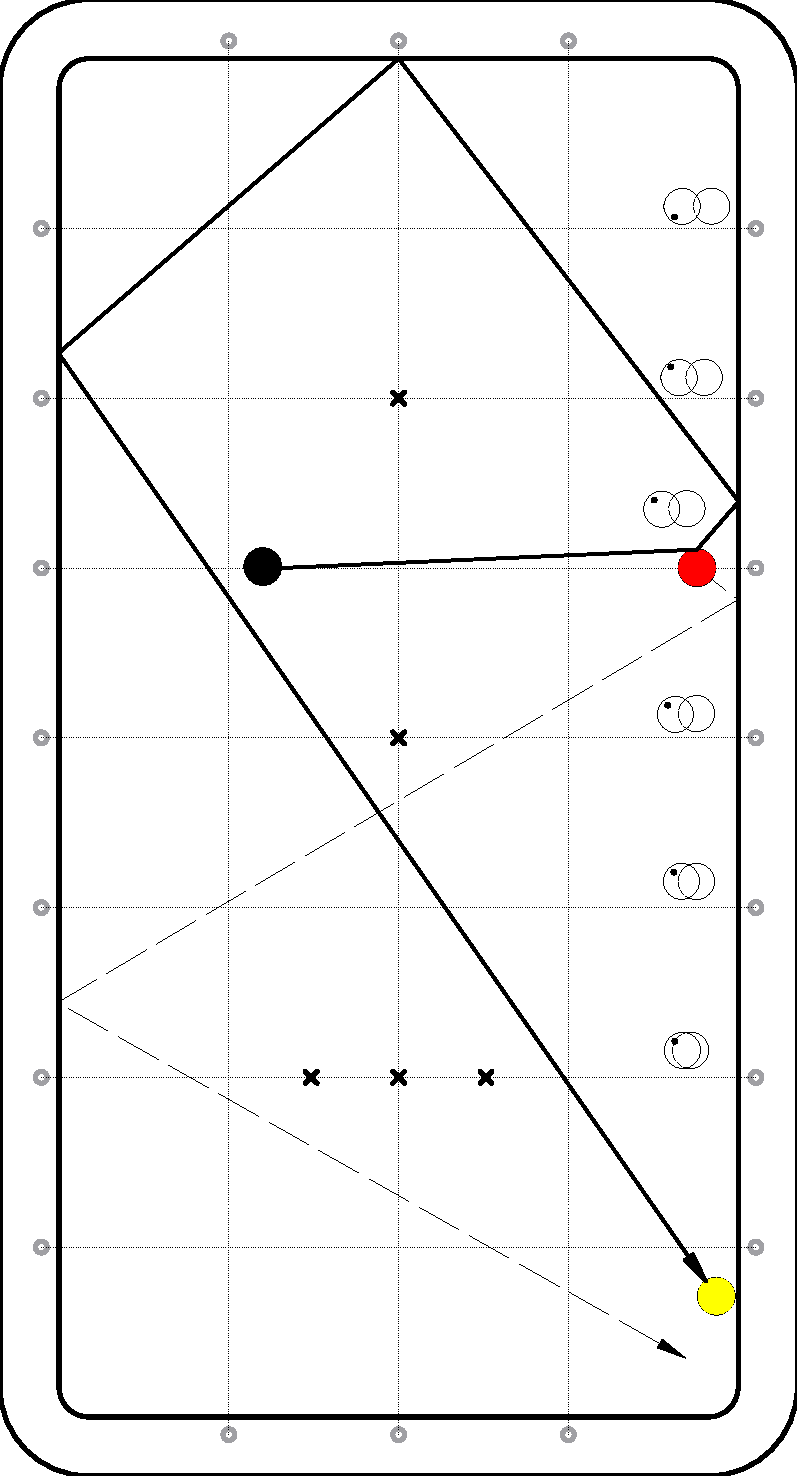
\includegraphics[width=0.85\linewidth]{A/imagesA/A19-01.pdf}
	\caption{Le Carrousel}
	\label{fig:a19-1}
\end{figure}
\clearpage

%% !TeX spellcheck = fr_FR
% !TeX encoding = ISO-8859-1

\section{Rappel par deux bandes}

Ce point semble facile et il l'est. Cependant, pour ramener la 2 dans le
� chapeau �, il demande une grande attention et un bon tour de main. Le
danger vient de la bosse possible de la 2 sur la 1, apr�s deux bandes.

Figure : le point se joue en trois quarts coul�, coup allong� et tr�s
accompagn�, peu ou pas d'effet favorable. La difficult� est la juste
prise de la 2. Prise trop fine, la 2 reste en chemin et ne rentre pas.
Prise trop grosse, la 2 risque de percuter la 1 en deux endroits : voyez
les croisements de trajectoires, particuli�rement le deuxi�me. Une bonne
allonge, donne un peu plus de vitesse � la 1 et permet de ramener sans
bosse.

Le tout est une question de mesure et ... d'entra�nement.

Entra�nement : Comme sur la figure, je conseille de commencer avec la 2
en face de la mouche 3. C'est cet emplacement qui est le plus dangereux
pour la bosse. Une fois cette position acquise, essayez des s�ries avec
la 2 en face de la mouche 2, puis en face de la mouche 1. Vous
constaterez par vous-m�me que plus la 2 est situ�e � haut �, moins
grosse (mais au moins une demi-bille) doit-elle �tre prise pour assurer
le point mais alors, la 2 rentre moins bien ! Pour quand m�me rentrer la
2, il y a deux solutions, soit allonger un peu moins ou jouer plus sec :
Ces derni�res nuances sont difficiles d'application surtout si on ajoute
que pour assurer le retour de la 2, la 1 arrive plus rapidement et
risque de ne pas rester dans le secteur, voire d'�clater la 3. Apr�s ces
brillants essais, on peut encore tenter le coup avec la 2 en face de la
mouche 4. C'est difficile et il ne faut pas descendre au-del�. Il s'agit
d'un vrai coul� sans effet, avec la 1 qui doit absolument passer devant
la 2 avant de toucher la petite bande oppos�e.

Cas particulier : Si la 3 est situ�e � une mouche du coin, le m�me coup
est encore possible avec un l�ger effet contraire haut de bille : plus
facile qu'il n'y para�t.

\begin{figure}[htb]
	\centering
	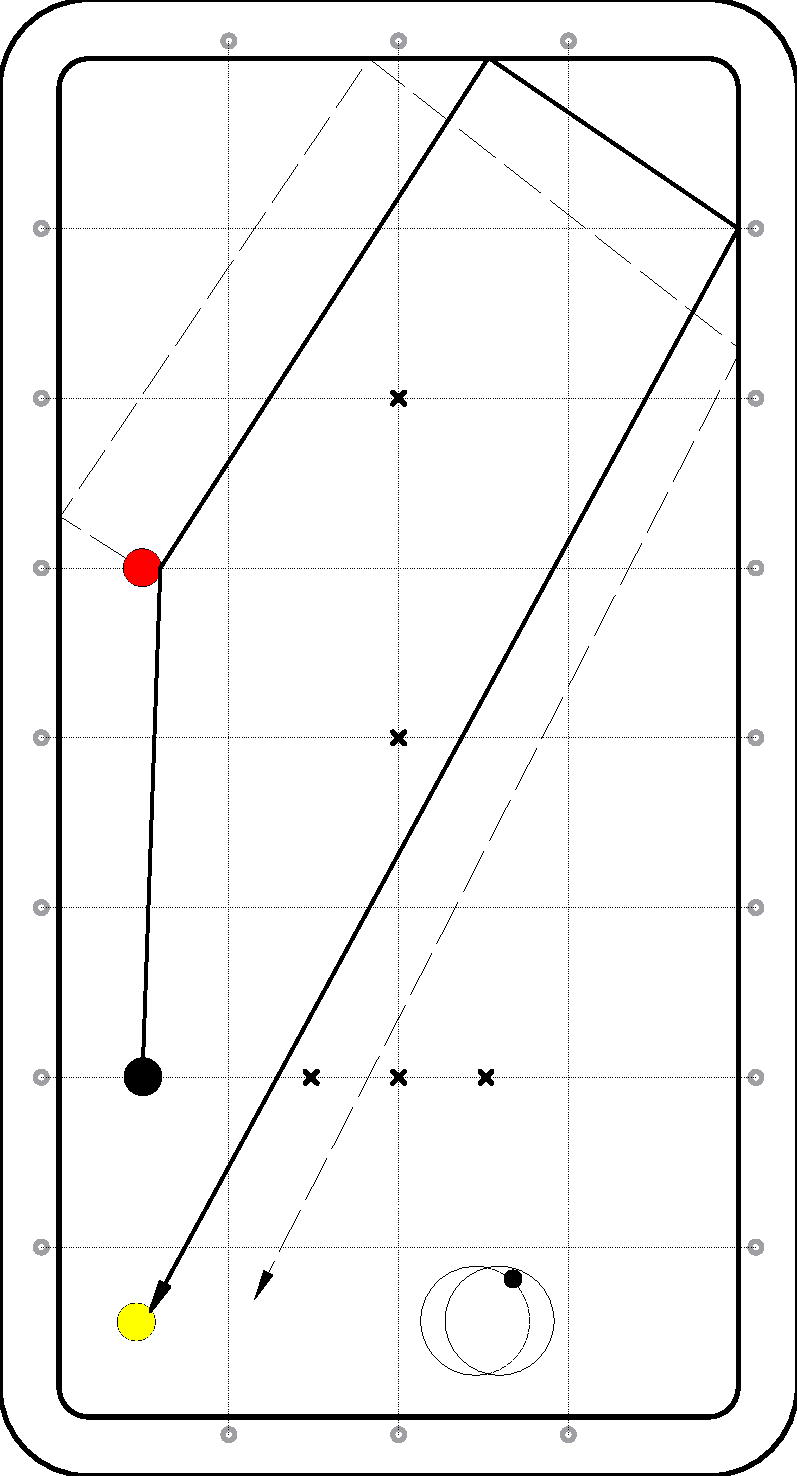
\includegraphics[width=0.85\linewidth]{A/imagesA/A20-01.pdf}
	\caption{Rappel par deux bandes}
	\label{fig:a20-1}
\end{figure}
\clearpage

%% !TeX spellcheck = fr_FR
% !TeX encoding = ISO-8859-1

\section{Le Point de Finesse}

Le point de finesse fait souvent peur. Quelques \textless{}\textless{}
trucs � peuvent aider � se donner confiance. Deux � grands cas � peuvent
se pr�senter :

Figure 1 : Les billes 2 et 3 sont tr�s proches l'une de l'autre et la 1
est �loign�e :

\begin{itemize}
	\item
	Examiner attentivement l'angle form� par les directions 2-3 et 1-2. Si
	cet angle est sup�rieur, �gal ou l�g�rement inf�rieur � 45� et si les
	billes 2 et 3 ne se touchent pas, jouez un simple 45�, c�d en
	demi-bille. En effet, il s'agit ici d'une fausse finesse. Si les
	billes faisaient les m�mes angles en �tant �loign�es l'une de l'autre,
	vous n'h�siteriez pas. Vous n'y verriez pas une finesse : n'en faites
	donc pas !
	\item
	Si l'angle pr�cit� est de 45� ou l�g�rement inf�rieur, vous pouvez
	jouer une demi-bille sur la 3 (!). Et oui, en visant une demi-bille
	sur la 3, la 1 touchera la 2 au passage. Votre fixation sur la 3
	�cartera la peur de viser sur la 2 ... (c'est un truc). Aucune
	inqui�tude � avoir. L'exp�rience le prouvera.
	\item
	Si l'angle pr�cit� est nettement inf�rieur � 45�, on peut encore
	rep�rer la portion de la 3 � toucher de mani�re � fr�ler la 2 au
	passage : donc encore rep�rer sur la 3.
\end{itemize}

Figure 2 : Les billes 1 et 2 sont tr�s proches l'une de l'autre.
Examiner d'abord, si la tangente commune int�rieure aux billes let 2
laisse la 3 bien visible ou bien la � coupe �, laissant visible, par
exemple, au moins une demi-bille � 30 cm. ou m�me moins, suivant la
facult� du joueur. En fait, c'est v�rifier qu'en jouant en ligne droite,
sans que la 2 n'op�re une d�viation de la 1, la 3 serait touch�e. Il
faut bien se dire dans sa t�te que la prise en finesse de la 2 est chose
ais�e. On s'attachera � jouer presque � c�t� de la 2, � la limite, visez
avec un seul ?il pour � prendre � le millim�tre qu'il faut et ... ne pas
regarder la 3 ... et jouer doucement pour ne pas accentuer l'angle ...
et ne pas mettre d'effet inutile ! On voit souvent des joueurs appliquer
un effet c�t� 2 : attention ! �a agrandit l'angle. Cet effet convient
lorsque vraiment trop proche de la 2, la pouss�e de la 1 risque de nous
faire faire un queut�. Dans ce cas oui, l'effet � contraire � fait
�viter le queut�. Mais attention, le bon effet provoque ce queut� car,
lors d'un touch� avec effet, le proc�d� reste en contact du c�t� oppos�
de l'effet appliqu� le temps d'une l�g�re d�viation de la bille pouss�e,
avant que celle-ci ne prenne la direction voulue, et on se trouve tout
�tonn� lorsqu'un arbitre nous arr�te pour ce que nous croyons �tre une
injustice alors qu'en fait, nous avons devant nous, un arbitre rigoureux
qui sanctionne notre distraction.

Remarque : Le point de finesse nous invite � jouer un point de vis�e sur
une bille en n�gligeant l'autre bille. Jouez doucement, de mani�re � ne
pas �vaser l'angle au moment du toucher ! Et surtout : ne pas avoir peur
!

\begin{figure}[htb]
	\centering
	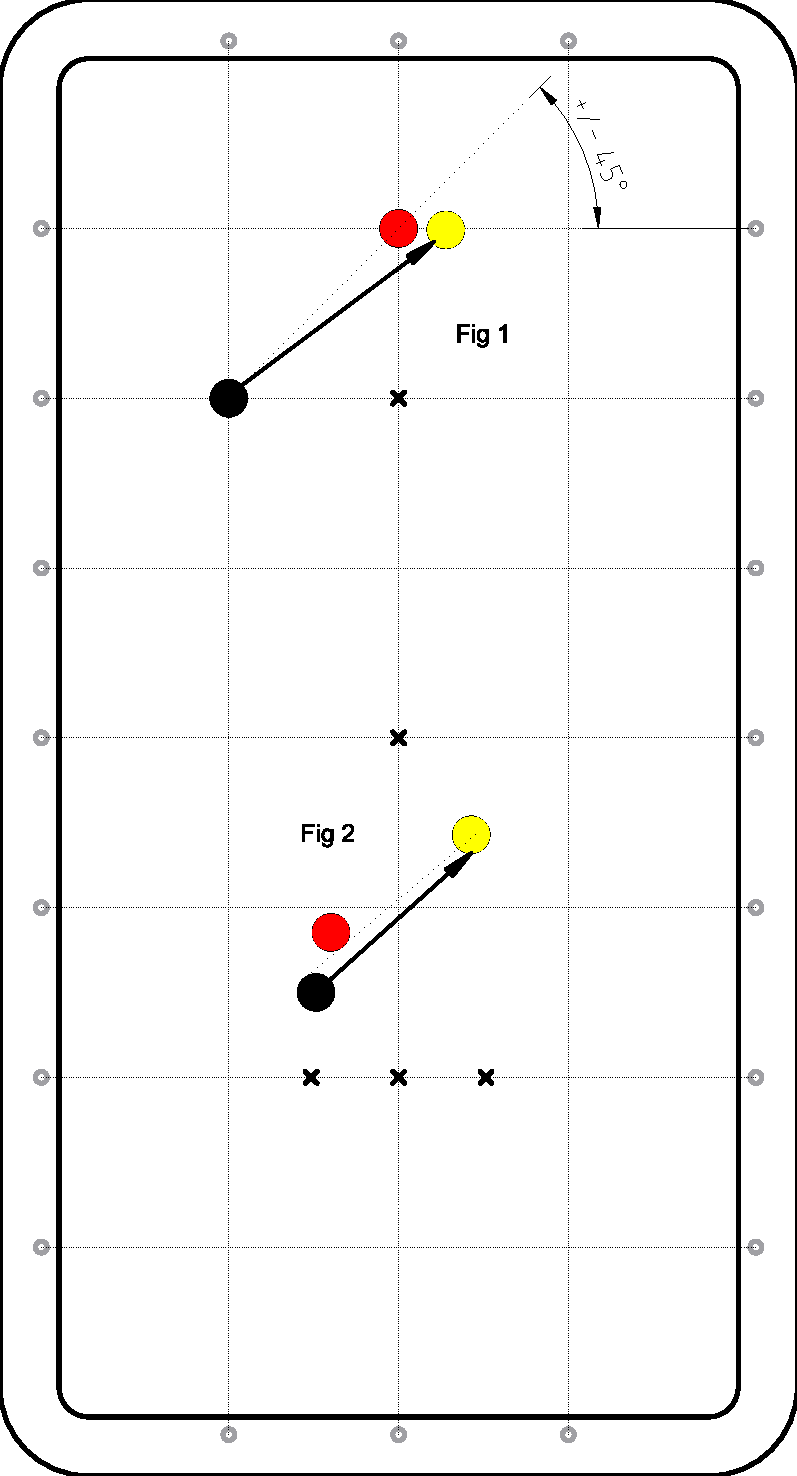
\includegraphics[width=0.85\linewidth]{A/imagesA/A21-01.pdf}
	\caption{Le Point de Finesse}
	\label{fig:a21-1}
\end{figure}
\clearpage

%% !TeX spellcheck = fr_FR
% !TeX encoding = ISO-8859-1

\section{Le long coul�}

Le long coul� fait souvent peur et on a raison. Il demande une grande
pr�cision et une tenue de canne ferme et bien rectiligne parce que le
coup port� est tr�s violent. La moindre erreur est multipli�e par un
facteur incertain.

Figure : dans ce cas, le coup est haut, tr�s allong� et tr�s fort,
violent m�me. L'effet est de pr�f�rence � droite avec une prise pleine,
avec seulement une nuance � droite. L'effet �carte un peu la 2 de la
trajectoire d'un contre �ventuel et la force du coup permet le rappel en
doubl� de la 2. Si la position des billes le permet, on peut aussi
appliquer un effet � gauche qui aura pour r�sultat de mieux serrer la 2
vers le jeu. Cependant, vu la difficult� du point, il est souvent
pr�f�rable de lui choisir un effet c�t� grande bande proche, ici �
droite. On augmente nos chances de r�ussite. Celui-l� fait s'�carter la
2 et si nous ne sommes pas tout � fait droit, deux cas peuvent encore se
pr�senter et nous sauver :

1 - : La 1 passe � gauche de la 3. Gr�ce � l'effet � droite, la 1 va �
casser � le coin derri�re par petite bande, grande bande et revient sur
la 2. La mise est sauv�e.

2- ; La 1 passe � droite de la 3. Gr�ce � l'effet � droite, la 1 ex�cute
un renvers� derri�re la 2 par la grande bande, petite bande et re-grande
bande avant de toucher la 2 par derri�re. La mise est encore sauv�e.

Remarque : gr�ce � l'effet, nous assurons une seconde chance de r�ussite
si la 1 passe � c�t� de la 2. C'est une double chance. Nous jouons avec
la possibilit� que les probabilit�s nous donnent. Ce point si difficile
devient un point de difficult� moyenne. Il ne faut cependant pas trop
tenter le diable. Si l'erreur est trop grande, la 1 ne se rattrapera pas
\ldots{} et la 2 non plus.

\begin{figure}[htb]
	\centering
	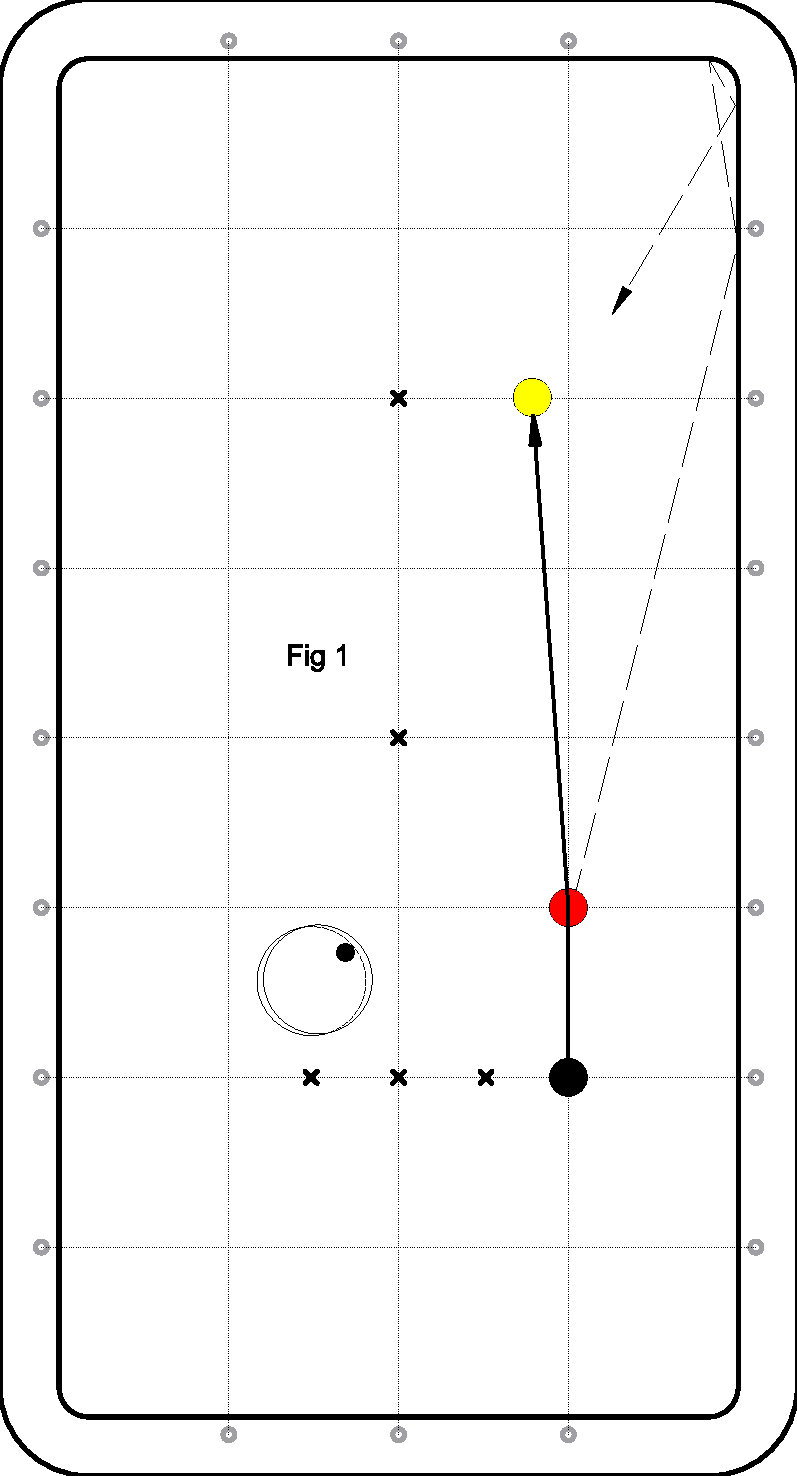
\includegraphics[width=0.85\linewidth]{A/imagesA/A22-01.pdf}
	\caption{Le long coul�}
	\label{fig:a22-1}
\end{figure}
\begin{figure}[htb]
	\centering
	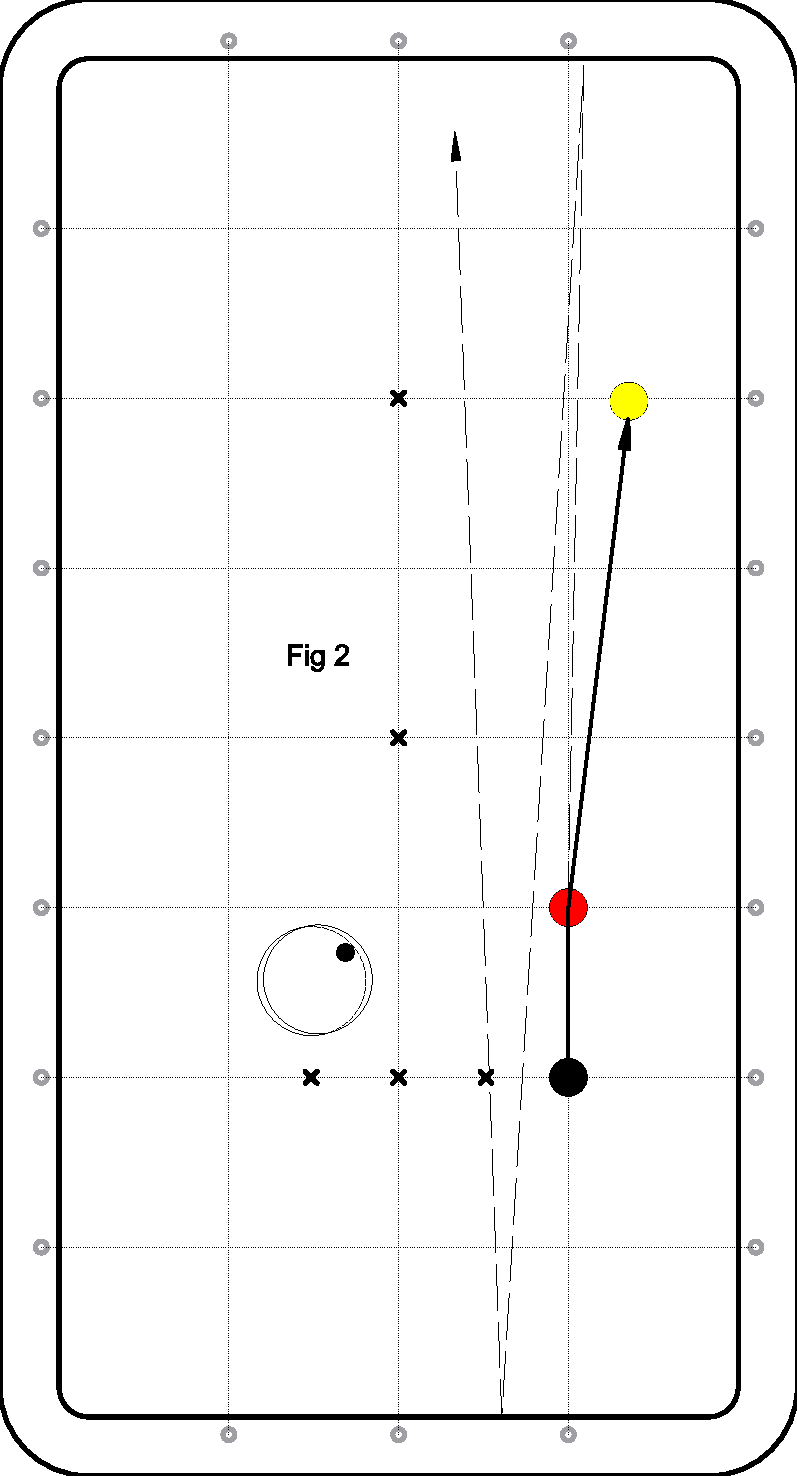
\includegraphics[width=0.85\linewidth]{A/imagesA/A22-02.pdf}
	\caption{Le long coul�}
	\label{fig:a22-2}
\end{figure}
\clearpage

%% !TeX spellcheck = fr_FR
% !TeX encoding = ISO-8859-1

\section{Petit R�tro - Long D�placement}

Ce petit point demande une bonne souplesse et une bonne confiance en
soi. La prise est celle d'un r�tro classique. Une r�gle ou bien un truc
� bien assimiler : plus la 2 est proche de la 1, plus la fl�che sera
courte, plus la 3 est �loign�e, plus la main arri�re est loin... Ce
n'est �videmment pas une r�gle absolue et vous verrez � l'usage, qu'il
est possible de la transgresser avec un bon r�sultat. Cette r�gle doit
vous aider � placer les mains sur la canne. La portion de la canne
comprise entre les mains et celle au-del� de la main arri�re constituent
un rapport calculable proportionnel � l'�nergie donn�e au d�part � la 1.
C'est donc tr�s important mais pour l'heure, nous appliquerons la r�gle
que j'ose r�p�ter : Petit d�placement : petite fl�che et long R�tro :
main arri�re loin... C'est ce qu'il faut appliquer ici, on l'aura
compris. On veillera � � bien laisser travailler �\textgreater{} la
canne elle-m�me, presque comme si les mains n'�taient pas l�, comme si
elles �taient l� uniquement pour soutenir la canne dans la bonne
direction sans la serrer ! Nous laissons travailler la canne (hum !)...
Quand on poss�de ce coup, le rythme de la 1 est assez spectaculaire,
comme si elle d�marrait seule, comme si elle avait une volont�. Avec
l'habitude et pour certains, le moelleux du mouvement charmera le
spectateur.

Entra�nement : Placer la 2 � 5 cm de la 1, puis 4, puis 3, puis 2, puis
1 et la 3 � 30 ou 40 cm � l'arri�re de la 2. Essayer des s�ries de 10 �
chaque distance jusqu'� une rentr�e en � chapeau � r�ussie � 90\%.
Essayer le retour � gauche et � droite. C'est fastidieux mais ce sera
payant. Remarque : Le queutage est tr�s dangereux. En fait, il y a
rarement queutage mais bien double touche. Que risque-t-il de se passer
? Au moment du toucher, la canne reste tr�s peu de temps en contact avec
la 1, le temps de parcourir 2 ou 3 millim�tres, tout au plus, rester
plus longtemps serait d'ailleurs consid�r� comme faute. Au contact de la
2, la 1 subit carr�ment un arr�t avant d'effectuer le r�tro. Si la canne
n'a pas �t� arr�t�e � temps, celle-ci re-percute la 1 en bas de bille et
la soul�ve. La 1 retouche alors la 2 sans avoir les � pieds au sol �
avec ce bruit caract�ristique bien connu des joueurs qui croient que ce
seul bruit constitue la preuve de la faute. Cela va tr�s vite et
souvent, le joueur lui-m�me ne sent pas le double coup.

Et l'arbitre ? : L'arbitre doit se placer de c�t�, de mani�re � bien
voir le mouvement de la 1. Ne pas se fier au bruit seulement ! Le bruit
doit constituer une confirmation de ce que l'?il a vu et ne constitue
pas seul, une preuve. Ce bruit provient du fait que la 1 et soulev�e.
Apr�s le choc de la 1 sur la 2, si la 1 s'arr�te, red�marre vers
l'avant, s'arr�te � nouveau, puis seulement effectue son mouvement
arri�re, il y a faute. En g�n�ral, si le point est tr�s court et fautif,
la 1 se soul�vera au deuxi�me contact de la canne. C'est tr�s visible vu
de c�t�. Le placement de l'arbitre est donc capital et les avis des
spectateurs experts qui se trouvent parfois loin de l'aire de jeu sont
souvent sans valeurs ; on les d�pistera facilement au fait qu'ils
affirment mais n'ont pas d'argumentation... Soyez ferme si vous avez ou
croyez avoir vu. Dans la majorit� des cas, il y aura toujours discussion
et ... mati�re � discussion.

\begin{figure}[htb]
	\centering
	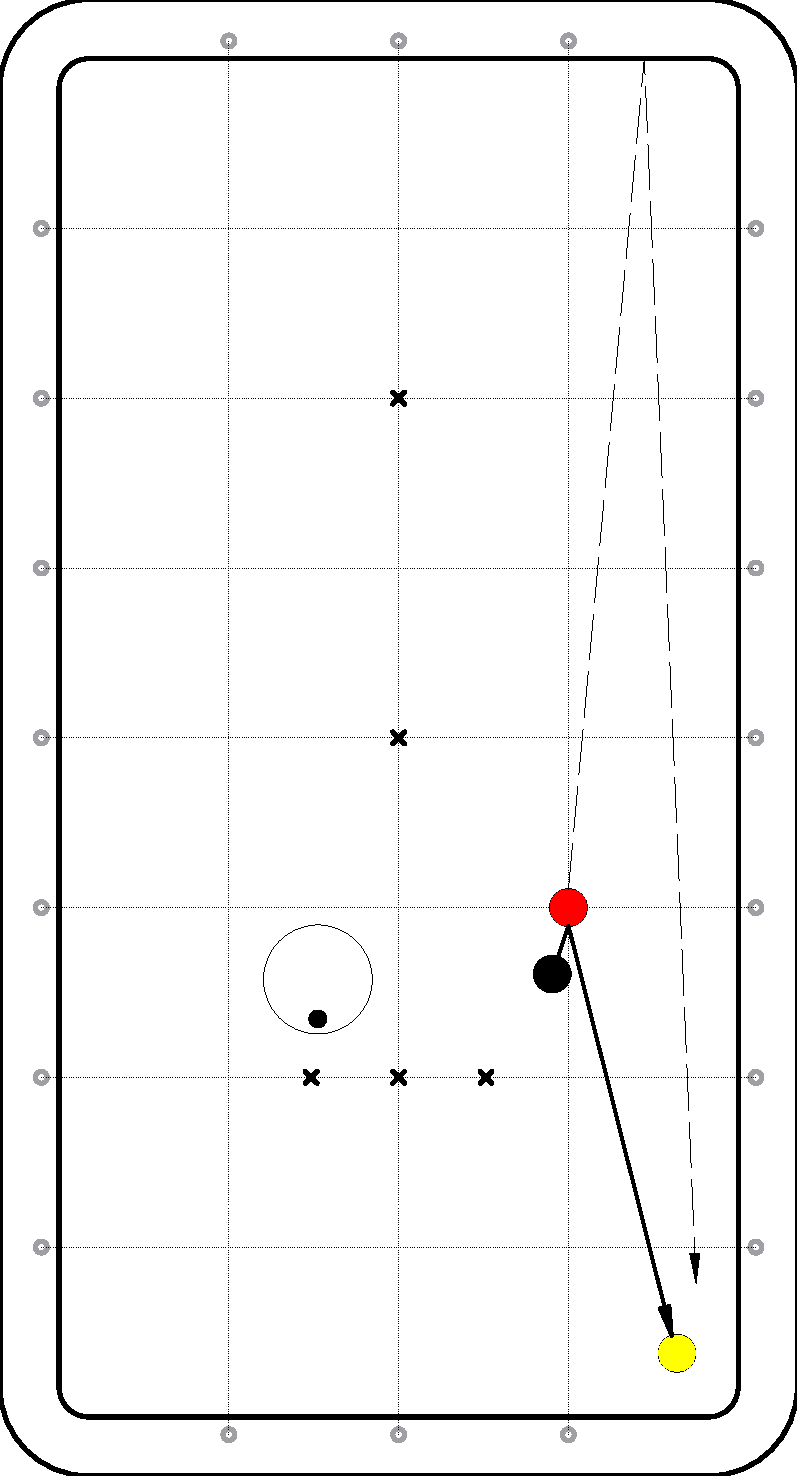
\includegraphics[width=0.85\linewidth]{A/imagesA/A23-01.pdf}
	\caption{Petit R�tro - Long D�placement}
	\label{fig:a23-1}
\end{figure}
\clearpage

%% !TeX spellcheck = fr_FR
% !TeX encoding = ISO-8859-1

\section{Le Point Mouche}

Dans tous les matches et � tous les modes de jeu, except� l'artistique,
ce point est le premier � r�aliser. La 1 doit obligatoirement percuter
la rouge en direct, c�d sans l'aide d'une bande. Le joueur peut d�cider
de faire placer sa bille de d�part sur la mouche gauche ou droite par
l'arbitre. Une partie commence par le � tir� � � bande. L'arbitre place
les billes des joueurs au niveau des mouches de d�part. Les deux joueurs
� tirent � vers la petite bande oppos�e. Au retour des billes, le joueur
qui poss�de la plus proche de la petite bande peut choisir s'il commence
ou s'il laisse la place � son adversaire. Attention, d�s que le � tir� �
est lanc�, la partie est commenc�e. Si le � tir� � n'est pas correct,
l'arbitre le fait recommencer. Les raisons d'incorrection sont multiples
: la bille d'un des deux joueurs a touch� la petite bande oppos�e avant
que la bille de son adversaire ait d�marr� ou bien les deux billes se
sont heurt�es ou bien une bille a touch� une grande bande ou bien une
des billes n'a pas touch� la petite bande oppos�e, etc. Par contre si un
� fantaisiste � trouve bien de � doubler � sa bille, le choix revient �
son adversaire. Apr�s le tir�, l'arbitre essuie encore une fois les
billes, les place sur mouche et d�clare la partie commenc�e... Bien que
ce point soit le seul qu'on est certain de rencontrer, il est souvent
rat�...

Le point mouche est difficile mais bien r�ussi, il donne d�j� une
possibilit� de s�rie. Aux trois bandes, il se joue un peu fort de
mani�re � allonger les trois billes le long d'une grande bande. Aux
autres modes de jeu, il se joue plus doux, plus souplement. Il faut
toujours l'essayer avant une partie pour reconna�tre les
caract�ristiques du billard. Laissons le trois bandes aux sp�cialistes.
C'est un coul� ! En th�orie, prendre la 2 en trois-quarts coul�. La 1
casse le coin gauche et revient par trois bandes. La 2 s'arr�te en bas
du billard. Le point se joue en trois bandes � s�ches � car, une fois la
3 manqu�e, la 1 ne reviendra jamais. Il y a risque de contre entre la 1
et la 2 le long de la grande bande droite. Ce contre est la preuve qu'on
avait pris la 1 correctement mais nous devons passer la main ! Ajoutez
une nuance haute ou basse selon qu'on a contr� par devant ou par
derri�re. En fait, il faut essayer selon la table ! De m�me, si on passe
au-dessus de la 3, allonger un peu, si on passe en dessous de la 3,
allongez moins. Mon truc : Je vise la 2 y pla�ant dans ma vis�e la
pointe de ma fl�che en tangence int�rieure c�t� gauche. Ensuite, je fais
glisser ma canne parall�lement � sa position de d�part jusqu'� pointer
au centre du secteur sup�rieur droit de la 1. Selon le r�sultat apr�s
l'essai, je vais rapprocher la fl�che du centre de la bille ou bien du
diam�tre horizontal ou les deux... Une fois le r�sultat correct, je
m�morise la position de ma fl�che par rapport � la bille 1 et
l'intensit� de p�n�tration (allongement). Ce point demande beaucoup
d'entra�nement jusqu'� ce que la 1 percute la 3 doucement .... (juste le
chemin) et que la 2 se blottisse � la petite bande. Composer avec tous
les param�tres en pr�sence n'est pas chose ais�e. Un long et acharn�
travail sera tr�s utile.

Bonne Chance !

\begin{figure}[htb]
	\centering
	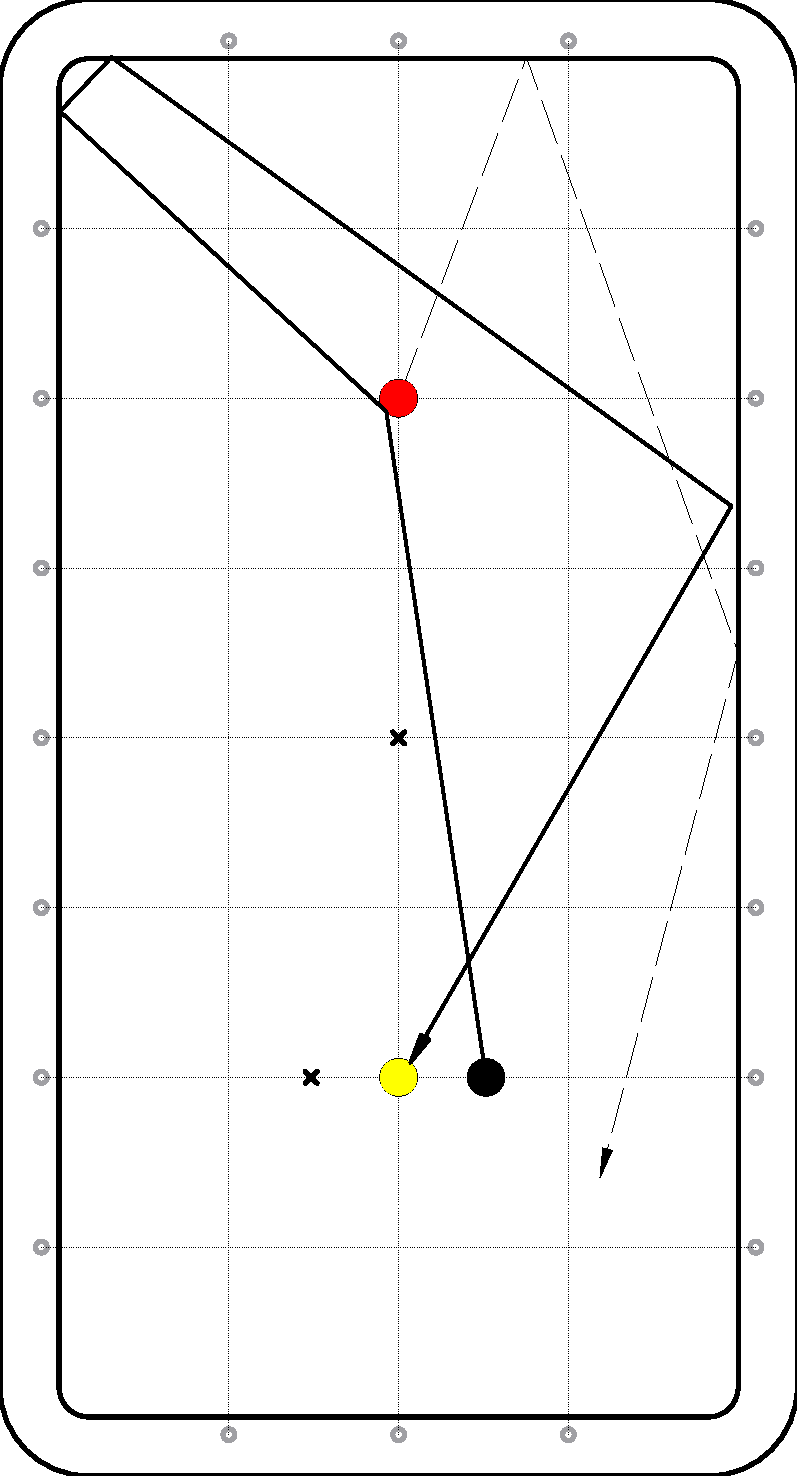
\includegraphics[width=0.85\linewidth]{A/imagesA/A24-01.pdf}
	\caption{Le Point Mouche}
	\label{fig:a24-1}
\end{figure}
\clearpage



\chapter{La technique}
\chapter{La queue lev�e}
\chapter{Les amortis}
\chapter{L'Am�ricaine}

\end{document}